\documentclass{report}


\usepackage[a4paper,margin=2cm]{geometry}
\usepackage{graphicx, color} % to include figures and colors
% \usepackage{hyperref} % for clickable references
\usepackage[round]{natbib} % get round brackets for citation
\usepackage[colorlinks=true,allcolors=blue]{hyperref} % for clickable references
\usepackage{amsmath} % normal text in math mode
\usepackage{float} % to force figure position
\usepackage{mathabx} % for earth symbol

\setcounter{secnumdepth}{3} % subsubsection numbering
\setcounter{tocdepth}{3} % subsubsection in contents

\usepackage{titlesec} % for subsubsubsection
\titleformat{\paragraph} % for subsubsubsection
{\normalfont\normalsize\bfseries}{\theparagraph}{1em}{} % for subsubsubsection
\titlespacing*{\paragraph} % for subsubsubsection
{0pt}{3.25ex plus 1ex minus .2ex}{1.5ex plus .2ex} % for subsubsubsection

\usepackage{siunitx} % scientific notation

\usepackage[titletoc,toc,page]{appendix} % for appendix format

\usepackage{amssymb}  % for real value notation
\usepackage{booktabs}  % fancy tables
\usepackage{multirow}  % multirow tables

\usepackage{arydshln}  % dashed lines
\makeatletter
\def\adl@drawiv#1#2#3{%
        \hskip.5\tabcolsep
        \xleaders#3{#2.5\@tempdimb #1{1}#2.5\@tempdimb}%
                #2\z@ plus1fil minus1fil\relax
        \hskip.5\tabcolsep}
\newcommand{\cdashlinelr}[1]{%
  \noalign{\vskip\aboverulesep
          \global\let\@dashdrawstore\adl@draw
          \global\let\adl@draw\adl@drawiv}
  \cdashline{#1}
  \noalign{\global\let\adl@draw\@dashdrawstore
          \vskip\belowrulesep}}
\makeatother   % dashed lines


\usepackage{tikz}  % graphical model
\usetikzlibrary{bayesnet}  % graphical model
\usetikzlibrary{arrows}   % graphical model
\usetikzlibrary{backgrounds}  % graphical model


\newcommand{\red}[1]{{\color{red}{#1}}}
\renewcommand{\bibname}{References}

\begin{document}
\begin{titlepage}



\newcommand{\HRule}{\rule{\linewidth}{0.5mm}} % Defines a new command for the horizontal lines, change thickness here

\center % Center everything on the page

 

%----------------------------------------------------------------------------------------

%	HEADING SECTIONS

%----------------------------------------------------------------------------------------




\includegraphics[width=\linewidth]{Titlepage/UvA-logo/uvalogo_regular_p_en.jpg}\\[2.5cm]

\textsc{\Large MSc Artificial Intelligence}\\[0.2cm]

\textsc{\Large Master Thesis}\\[0.5cm] 



%----------------------------------------------------------------------------------------

%	TITLE SECTION

%----------------------------------------------------------------------------------------



\HRule \\[0.4cm]

{ \huge \bfseries Detecting Exoplanet Transit Signals in Light\\ Curves Using Recurrent Neural Networks}\\[0.4cm] % Title of your document
% { \huge \bfseries Detecting exoplanet transit signals in light\\ curves using recurrent neural networks}\\[0.4cm] % Title of your document

\HRule \\[0.5cm]


 

%----------------------------------------------------------------------------------------

%	AUTHOR SECTION

%----------------------------------------------------------------------------------------



by\\[0.2cm]

\textsc{\Large Yke Jan Rusticus}\\[0.2cm] %you name

11306386\\[1cm]





%----------------------------------------------------------------------------------------

%	DATE SECTION

%----------------------------------------------------------------------------------------



{\Large \today}\\[1cm] % Date, change the \today to a set date if you want to be precise



48 ECTS\\ %

October 2020 -- August 2021\\[1cm]%



%----------------------------------------------------------------------------------------

%	COMMITTEE SECTION

%----------------------------------------------------------------------------------------

\begin{minipage}[t]{0.4\textwidth}

\begin{flushleft} \large

\emph{Supervisor:} \\

MSc D. \textsc{Ruhe} % Supervisor's Name

\end{flushleft}

\end{minipage}

~

\begin{minipage}[t]{0.4\textwidth}

\begin{flushright} \large
% \begin{flushleft} \large

% \vspace{-3pt}\emph{Mentor:} \\
\vspace{-3pt}\emph{External co-supervisors:} \\

Prof. Dr. B. H. \textsc{Foing}\\
Dr. A. M. \textsc{Heras}\\

\end{flushright}
% \end{flushleft}

\end{minipage}

~

\begin{minipage}[t]{0.4\textwidth}

% \begin{flushright} \large
\begin{flushleft} \large

\vspace{-3pt}\emph{Assessor:} \\

Dr. P. D. \textsc{Forr\'{e}}\\

% \end{flushright}
\end{flushleft}

\end{minipage}\\[2cm]



%----------------------------------------------------------------------------------------

%	LOGO SECTION

%----------------------------------------------------------------------------------------



% \framebox{\rule{0pt}{2.5cm}\rule{2.5cm}{0pt}}\\[0.5cm]


\includegraphics[width=4.5cm]{Titlepage/ESA-logo/esa-logo.png}\\ % Include a department/university logo - this will require the graphicx package

% \textsc{\large European Space Agency}\\[1.0cm] % 

 

%----------------------------------------------------------------------------------------



\vfill % Fill the rest of the page with whitespace



\end{titlepage}

{
  \hypersetup{linkcolor=black}
  \tableofcontents
}

\chapter{Introduction}
\label{chap:introduction}

The discovery of exoplanets is the first step in answering a broad range of fundamental questions. Is our solar system one of a kind? Is there life elsewhere in the universe? Exoplanets, short for extrasolar planets, are planets orbiting stars other than our Sun. It was only after the 90's that scientists became certain of their existence and nowadays more than 4000 examples are known\footnote{\url{https://exoplanetarchive.ipac.caltech.edu/docs/counts_detail.html}}. Several approaches to exoplanet discovery exist, the most successful of which is the transit method. This method relies on the rare event that a planet moves in front of its host star with respect to our line of sight, an event that occasionally occurs for Mercury and Venus. Transits express themselves in the form of periodic dips in the observed brightness of a star over time.  The detection of these dips in stellar data is therefore essential to the discovery of new exoplanets. 

In the following sections, the problem of detecting transit signals is described in further detail, as well as the motivation to approach this problem from different perspectives. Common approaches and limitations are given, to shape our understanding of how the solution to this problem could benefit from artificial intelligence (AI). The contributions and outline of this work are given in the last sections of this chapter.

\section{Problem}

Different approaches to exoplanet discovery exist. This work focuses on the transit method, the most successful method in terms of number of discoveries. The transit method relies on the rare event that a planet moves in front of its host star in our line of sight, i.e. the so-called ``transit''. Transits express themselves in the form of periodic dips in the observed brightness of a star over time. The detection of these dips in stellar data is therefore essential for the discovery of new exoplanets. 

The observed brightness, or flux, of a star over time is referred to as the star's ``light curve''. Generally, transit signals have a duration in the order of hours and light curves have a time span in the order of days or months. A transit signal may repeat itself if the orbital period of the exoplanet is shorter than the time span of the light curve. In case the orbital period longer, a transit signal may occur only once, in which case we speak of a ``monotransit''. Moreover, multiple planets might orbit the same star, in which case we can have multiple transit signals from different planets in the same light curve.

The physics of transits is well-understood, but the detection of their signatures in light curves is hindered by stellar and spacecraft induced noise. In addition, transit signals may vary in depth, duration and general shape depending on stellar and planetary parameters. Furthermore, transit signals are in general weak and sparse, so the chance of any given light curve to contain detectable transit signals is low. A detailed description of the challenges and their origins is given in Section \ref{sec:challenges}.

The problem we address is thus the detection of dips in light curves of stars that could indicate the presence of an orbiting exoplanet. In literature, however, some ambiguity exists in the naming of different steps in the process of discovering transiting exoplanets. In the detection step, i.e. the focus of this thesis, we search for potential signals in a light curve, and provide parameters such as the epoch $t_0$ and orbital period $P$ of the detected candidates. The epoch is a reference time, e.g. the time of the first transit event in the light curve, which together with $P$ allows for retrieving the signal that was found. Detection should not be confused with identification or vetting, the step in which the detected signals are classified as false positive, planet candidate, or candidate of another type of object.


\section{Motivation}

Within the course of a few decades, the status of exoplanets has changed from hypothetical to common. The discovery of exoplanets has greatly enriched our view on the universe, as with each new discovery we can better answer questions regarding, for example, the distribution of exoplanet compositions or planetary system dynamics and evolution. Nevertheless, though several candidates have been identified, the search for a second Earth is still going, and with that the search for life. The general motivation to search for more exoplanets is thereby clarified. 

However, as mentioned, several approaches to exoplanet discovery exist. Each method has its own benefits and drawbacks, for which we refer the reader to Section \ref{sec:disc_methods}. This thesis focuses only on the transit method, which is motivated by several reasons. The first is that the problem to solve is relatively straightforward, i.e. detecting dips in brightness over time. Second, plenty of data is available, because the only thing to be measured is the brightness of stars over time, which can be done at a single wavelength interval for many stars simultaneously. Last, a transit signal carries a wealth of information about the planetary system at hand. For example, the depth of the signal is related to both the size of the planet compared to it's host star and several orbital parameters such as the inclination, the angle of the orbital plane orbit relative to the observer. The periodicity of the signal directly tells us the orbital period of the planet, although the duration of a single transit signal also constrains this parameter. More information about the transit method and what we can learn from it is given in Section \ref{sec:transit_method}. 

Before we can determine all these parameters, however, the signal need to be detected. Several algorithms exist to search for transit signals in light curves, but as each algorithm can differ, so can their returned detections. One algorithm may miss a planet that an other algorithm finds and vice versa. For this reason, in this thesis we aim to develop a new transit detection algorithm, which works substantially different from existing methods.




\section{Common approaches and limitations}
\label{sec:approaches}

Most commonly used in the task of transit detection is the Box Least Squares (BLS) algorithm \citep{kovacs2002box}. This algorithm uses a box-shaped model of a strictly periodic signal. In order to search for transits, the model is fitted to the data at different signal durations, periods and epochs. Variants to this algorithm exist, for example Transit Least Squares (TLS) \citep{hippke2019optimized}, or Sparse Box Least Squares (SBLS) \citep{panahi2021sparse}.

One limitation of these methods is their requirement of a detrended input light curve. Detrending is the process of removing irrelevant time-dependent noise from the light curve. In the process, however, information is altered at short time scales, so the signal that we wish to find may get reduced or altered \citep{hippke2019wotan}.  Alternatives have therefore been proposed, for example simultaneously modeling the background while searching for transit signals \cite{foreman2015systematic}.

However, what these methods still have in common is their brute-force approach to searching for signals. 
They rely on iterating through trial configurations of parameters that define the signal's shape and timing. In particular for transit models more realistic that the box-function, this iteration over potential signals can be costly. In addition, in case the search is directed towards multiple planets in the same light curve, this process has to be repeated several times, each time masking the previous signal that was found. Furthermore, the model configurations to be iterated over are generally specified by the user, which might cause the search to be biased towards specific signal shapes.

An approach based on AI may overcome several of these limitations, as shown by \cite{pearson2018searching}. In their work, the use of a one-dimensional convolutional neural network (CNN) is proposed for the task of transit detection. On the one hand, neural network outputs can be more difficult to interpret than outputs of box-fitting algorithms, because a neural network generally has complex hidden dynamics which make it function like a ``black box''. On the other hand, they come with several benefits. The CNN does not iterate over transit shapes, and detrending the input light curve is not necessary. 
In the proposed method, however, the CNN is only capable of providing a single output for an input light curve segment of fixed size. 
This means that it cannot directly be applied to a full-length light curve of arbitrary size, and we need to take additional steps to determine the timing of potential signals. One option is to apply the CNN to overlapping segments in the light curve to obtain outputs at each time step. However, this approach makes the CNN less intuitive and efficient in its use for detection. 

In the task of transit signal detection, the use of recurrent neural networks (RNNs) remains unexplored. 
The question therefore remains whether RNNs can provide an efficient and competitive alternative to classical transit detection methods, and improve over CNNs in terms of their applicability. Additionally, we raise the question of how the outputs of RNNs can be made more intuitive for the task of detection. 



\section{Summary of contributions}
\label{sec:contributions}

This work reports the first attempt in literature of using RNNs for the task of transit detection. The research presented revolves around the question of whether and how RNNs could be applied to compete with conventional transit detection algorithms. We provide a detailed analysis of what preprocessing steps could be considered when applying this network to light curves to search for signals. Successes and failure cases of our method are identified, and the general performance is evaluated in comparison to existing approaches. Our approach does not require detrending of input light curves as opposed to commonly used methods. During search, the RNN does not iterate over transit durations, depths or other parameters that define the signal's shape, since the model is implicitly trained to recognize these features prior to application. 

In short, we found that the RNN copes better with longer input light curves than the CNN. This is important for the task of detection, as light curves are generally large in size. In a series of experiments imitating real-world problems, we found the RNN to show most potential in the task of monotransit detection, because it does not rely on periodicities of signals and it can be applied highly efficiently. It outperformed the box-fitting algorithm of \cite{foreman2016population} in the task of retrieving 2500 single transit events from a set of 5000 simulated light curves. The RNN achieved an  average precision (AP) of 0.43, while the baseline achieved an AP of 0.35. In the case of multiple transit signals in a single light curve, we found the BLS algorithm to benefit more from the periodicity of the signal, as it outperformed our RNN-based algorithms. In the task of retrieving 2500 planets with repeating transit signals from 5000 light curves, the best RNN-based algorithm achieved an AP of 0.59 and BLS an AP of 0.66. In both cases however, the algorithms tested were able to detect signals that the other one was not able to find. In other words, the methods performed complementary. This result suggests that an RNN-based transit detection method could open the door to detecting exoplanets that would otherwise be overlooked by conventional algorithms.

\section{Outline}

Since the problems and challenges in exoplanet science differ substantially from more ``typical'' AI-problems encountered on Earth, a large part of Chapter \ref{chap:background} is devoted to create a common ground. Exoplanets are described in further detail, as well as some noteworthy discoveries, discovery methods and facilities. A detailed description of the challenges of detecting transit signals is given, and we discuss previously proposed approaches to the problem. Furthermore, we discuss work on AI applied to different problems in exoplanet science, and other related work. Chapter \ref{chap:methodology} describes our proposed method, as well the simulated data that was used in the experiments. In Chapter \ref{chap:experiments}, the RNN-based detection algorithm is evaluated and compared to other methods, of which the main baseline is based on the Box Least Squares algorithm \cite{kovacs2002box}. The results are discussed in Chapter \ref{chap:discussion} and in Chapter \ref{chap:conclusions} the main conclusions are listed and the work is summarized.


\chapter{Background}
\label{chap:background}

\red{[TODO]}

\section{Exoplanets}

Most people are familiar with the planets in our solar system, e.g. Venus, Mars, Jupiter. What these planets have in common is that they all orbit the same star, that is our Sun. Exoplanets might be similar to the planets we know well, but they orbit different stars, which makes them hard to find and difficult to study.

\subsection{A brief history of exoplanet science}
For a long time, Earth was one of the few planets known to human kind, as part of the only planetary system known. However, billions of stars exist within our galaxy alone, each potentially with their own orbiting exoplanets. [TODO: list discoveries] Later on, more exoplanets were discovered, and thus the list of known planetary systems was extended. 


\subsection{Discovery methods}
Exoplanets are not as straightforward to observe as planets in our own solar system. For example for Mars or Jupiter, light reflected from the planet's surface can be observed with the unaided eye. To observe Neptune, a small telescope is sufficient. For exoplanets however, the distances between stars play a role. Distances between planets and their host star are small compared to the distances between stars. The distance between Earth and the Sun is 1 Astronomical Unit (1 AU = \num{1.496e8} km) and the distance to the nearest star is about $10^5$ AU. First of all, this means that any exoplanet will thus be much farther away than the planets in our solar system. Second, we cannot observe exoplanets in isolation from their environment as we can do with planets in our solar system [TODO: include the exception of rogue planets]. Nevertheless, several methods have successfully been used to discover exoplanets, a few of which are listed below.

\subsubsection{Transit method}
\red{[TODO: describe the requirement for an edge-on system]}.\red{ [TODO: describe periodicity and transit shapes in general]}.
The most successful method in terms of number of discovered exoplanets is the transit method. This method forms the basis of this thesis. As illustrated in Figure \ref{fig:transit}, an exoplanet can move between the observer and the star it orbits. If the observer measures the brightness of that star over time, a dip is observed in the resulting \textit{light curve}. The depth of this transit signal depends on the relative size of the planet compared to its host star. If the radius of the star is given by $R_*$, then the stellar disk has a surface area of $\pi R_*^2$. During transit, the exoplanet blocks the star light that is emitted from an area of $\pi R_{p}^2$ from the stellar surface, where $R_{p}$ is the planet's radius. Therefore, during an ideal transit, a a fraction $R_{p}^2/R_*^2$ of the star's emitted light is blocked by the exoplanet.

% \begin{figure}
%     \centering
%     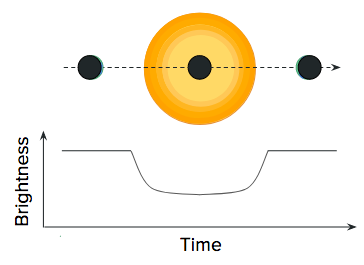
\includegraphics[width=0.3\linewidth]{Introduction/Figures/transit.png}
%     \caption{[TODO: use DejaVu Sans font for labels], [TODO: change planet color to black, because it should not be visible]}
%     \label{fig:transit}
% \end{figure}

\subsubsection{Transit timing variations}
\red{[TODO]}

\subsubsection{Radial velocity}
\red{[}This is arguably the most intuitive method\red{]}, as it aims to directly image a planet and resolve it from its host star. Although the idea is simple, in practice this method is challenged by the fact that the observed light from distant planetary systems is greatly dominated by the light emitted by the host star.
\subsubsection{Direct imaging}
By observing the light of a star at different wavelengths, its radial velocity can be inferred from shifts in the resulting spectrum. A change in radial velocity over time can be explained by the mutual interaction between an orbiting body and the star, causing the star to to move back and forth slightly in our line of sight. This method can also constrain the masses of the objects within the system.
\subsubsection{Microlensing}
A microlensing event occurs when a compact body such as a star acts as a lens and magnifies a more distant object in the background. This is due to the fact that the path of a ray of light is bent when it passes a massive body. In case a foreground star passes a background star in our line of sight, this effect should be visible for some duration as a peak in their combined brightness. Based on the signature of this change in brightness, one could infer whether a planet is likely to orbit the foreground star.

\subsection{Exoplanet-hunting missions}
Since the discovery of the first exoplanets, the rate at which exoplanets are detected has taken an exponential boost. Where at first it was the radial velocity method, it is now the transit method that holds most discoveries. At the time of writing, about one exoplanet is discovered every day over the past ten years on average by using the transit method. For all other methods combined, on average about one exoplanet is discovered every six days. The major turning point was when the search for transiting exoplanets was taken into space, and stars were monitored by the hundred thousands.

\subsubsection{Ground-based surveys}
\red{[TODO]}
\subsubsection{CoRoT}
\red{[TODO]}
\subsubsection{Kepler and K2}
With over 2500 exoplanet discoveries, Kepler and its continued mission ``K2'' are responsible for the detection of more than half of the known exoplanets. The Kepler space telescope has observed half a million stars in a small section of the sky. For most targets the cadence, or observation interval, was 30 minutes. A small fraction was observed with a cadence of one minute. Kepler operated for nearly ten years. Since its retirement in 2019, Kepler data is still a source for exoplanet discovery, as hidden and previously overlooked transit signals may yet to be detected \citep{hedges2019four}.

\subsubsection{TESS}
Launched in 2018, the Transiting Exoplanet Survey Satellite (TESS) has taken over the work of Kepler. As opposed to Kepler, TESS observes the full sky during its mission in the search for transiting exoplanets. It observes more brighter and closer targets than Kepler. TESS observations are of 2-minute cadence, though some targets are observed with a cadence of 20 seconds. Every 27.4 days, or sector, TESS changes its field of view. About halfway through each sector TESS links data down to Earth, during which no observations are made. At the time of writing, 125 exoplanet discoveries have resulted from TESS observations. With already over 200.000 stars observed, TESS is expected to discover thousands more.

\subsubsection{PLATO}
The PLAnetary Transits and Oscillations of stars (PLATO) mission will increase the numbers of several aspects. Planned for launch in 2026, this space-based telescope consisting of 34 \red{[TODO: fix, is less]} individual cameras will monitor up to a million stars. Its mission is to discover new transiting exoplanets and study their properties in greater depth. It will also perform asteroseismology to determine stellar parameters such as their mass. In combination with radial velocity measurements from the ground, this will allow for better characterization of the unknown worlds.

\section{Process of discovering transiting exoplanets}
Observing a transit event is one thing, finding the transit signal in a light curve is another. This task is simple if the existence of a planet is known beforehand, but this is not true in our case, so we need to search for signals. Once potential signals have been detected, the process continues, as the nature of each signal needs to be validated. The steps from raw light curves to the discovery of new exoplanets are described in the following subsection, after which follows a detailed description of the challenges that need to be overcome in the process.

\subsection{Detection, identification and characterization}
\label{sec:disc_process}

Apart from preprocessing the light curves, the detection of transit signals is the first step in the process of discovering transiting exoplanets. In literature, however, some ambiguity exists between the detection step and the step that follows detection. We follow the categories used by  \cite{jaratransiting} (as well as other works) and emphasize the difference between detection and identification.

In the detection step, which is the focus of this thesis, transit signals are blindly searched for without prior knowledge of their timing, shape or existence in general. Epoch $t_0$ and period $P$ (if applicable) and possibly other parameters of potential signals are determined and passed to the next step.

Identification, or vetting, is the processes of ruling out clear false positives from the returned detections. Often this is a binary classification task, where the isolated transit signal is classified as planet candidate or false positive. The main difference with the detection step is that during identification, no new potential signals are being searched for. Admittedly, one could apply an identification model to every part of a given light curve to search for new signals, although in most cases this is not what the algorithm was designed for. Furthermore, this would likely results in an unnecessarily inefficient detection algorithm.

Once a potential signal has passed the identification step, this still does not mean we have found a new planet. According to \cite{akeson2013nasa}, a candidate exoplanet must meet the following criteria to be included in the Exoplanet Archive: (1) it has a (minimum) mass estimate of no larger that 30 Jupiter masses, (2) its properties are described in the peer-reviewed literature, and (3) sufficient follow-up observations and validation have been undertaken to deem the possibility of a false positive as unlikely. For example, after the transit method is applied, one could attempt to confirm and characterize the system further using radial velocity measurements, or more accurate modelling techniques.


\subsection{Challenges}
\label{sec:challenges}

Although a transit signal is clearly defined, it is often a difficult task to detect or study them. This is mostly because the signals are usually weak and the background varies at greater amplitudes than the signal. These and other challenges are explained in detail in the following subsections.

\subsubsection{Small chances and weak signals}

For the transit method to work, a planetary system is required to be oriented edge-on (i.e. with an inclination $i \approx 90^\circ$). If the system is seen face-on ($i \approx 0^\circ$), any orbiting planet would not transit its host star with respect to our line of sight. However, no mechanism restricts planetary systems from being oriented randomly, so even if all stars would have orbiting planets, a large portion would go undetected. The chance of a planet transiting also depends on the distance from its host star. The farther away from the stars, the smaller the chance of a planet transiting.  If one were to observe our Sun from far away, the chance that Earth would transit the Sun for a random orientation of our solar system is only 0.47\%. Furthermore, even if it would transit, its 13-hour signal would only repeat once per year and leave a dip in the Sun's observed brightness of only about 80 ppm, or 0.0008\%. Hence, the transit method is biased towards detecting short-period Jupiter sized planets, as these cause transit signals that are more frequent and more profound. Nevertheless, the goal is also to detect Earth-like planets, which are small and have larger distances from their host star. For this to succeed, the background flux needs to be accurately modeled in order to disentangle it from the transit signals.

\subsubsection{Stellar activity}

Part of the reason why the background flux in a light curve is not constant is due to stellar activity. Stars, like our Sun, are not uniform spheres that emit a constant amount of photons at all times. First of all, starspots could be present. These visually dark regions on the stellar surface are relatively low in temperature, and thus decrease the flux. On the other hand, higher temperature regions can increase the flux. This alone would be no problem if the spots would always be present. However, starspots come and go with a lifetime depending on their size. Moreover, the star itself can be rotating, with the result that any spots that are present come in and out of sight as it rotates. This effect is called rotation modulation. 

To complicate things further, a star's surface is dominated by cell-like structures called granules, which are caused of energy transport below the stellar surface. As hot and thus brighter plasma rises, cooler and dimmer plasma descents, leaving the stellar surface as a constantly changing with a fluctuating brightness. These effects can closely mimic transit signals in a light curve, and thus often lead to false positive transit detections. Other stellar activity includes for example, stellar oscillations and sudden outbursts of energy, or flares.

In summary, a light curve may exhibit quasi-periodic patterns that are caused by complex mechanisms at local and global scales on and below the stellar surface. \red{[TODO: compare amplitudes of fluctuation with transits, see \cite{barros2020improving}]}.

\subsubsection{Instrumental and photon noise}

No instrument is perfect, neither is the setup of the observations. For ground-based observatories, weather could play a role or measurements might be affected by stray light from nearby cities. In this thesis, we assume all data to be coming from space-based observatories. These are not affected by the obstacles mentioned above, but still have imperfections. For example, temperature changes in the spacecraft can alter the pointing of the telescope, resulting in jumps or drifts in the observed flux from stars. As the telescope typically observes thousands of targets at the same time, this affects all the thousands of corresponding light curves, though potentially in slightly different ways. And although stray light from cities plays less of a role in space, stray light from the moon may still negatively influence the quality of measurements.

Poor quality data is often filtered out, leaving gaps in the resulting light curves. This could pose a problem for certain data processing algorithms. Larger gaps could result from when the spacecraft downlinks data back to Earth. During this process, the telescope might not gather new data, causing the light curves to have gaps of several hours to a few days.

Another source of noise, although not due to instrument imperfections, is photon noise. This type of noise originates from the arrival of different amounts of photons at the detector between different observations. The number of arrivals per observation can be modeled as a Poisson distribution, which for a large number of photons approximates a Gaussian distribution. The photon noise can thus often be seen as the time independent white noise in the data.

\subsubsection{Astrophysical false positives}

Sometimes, a false positive detection is not due to stellar or spacecraft induced noise, but due to other phenomena. For example, a large portion of the stars exists in a binary configuration. In case an eclipsing binary (EB) system is seen edge-on from Earth, the stars transit each other just like an exoplanet would transit its host star. Generally, the corresponding transit signals will be larger than for exoplanets, but if the stars' orbital plane is slanted and they have grazing transits, the signals can become more similar to exoplanet transits. 

More similar to exoplanet transit signals can be due to an EB system lurking in the background of an observed star. These background EBs (BEBs) can be much farther away than the star under consideration, but contribute to the star's light curve. The BEB transit signals will thus also be smaller and could mimic exoplanet transit signals in the light curve of the foreground star.

In the detection step, however, it is not the main goal to discern (B)EBs from exoplanet transit signals. This can well be done in the identification step. Similarly, the detection step could return a signal that is in fact 
caused by a large exocomet or asteroid. Restricting our detection algorithm too much on what kind of signals it is allowed to pick up, may exclude various interesting signals. In many cases, however, it would be of great astrophysical value to study those signals.

\subsubsection{Transit signal shapes}

The basic shape of a transit signal is determined by a set of parameters. These parameters include, among others: the orbital period of the planet, its radius relative to its host star, the distance from its host star, the inclination of its orbital plane and the eccentricity of its orbit. Each of these affects the transit shape differently, e.g. the inclination determines if the signal will be U-shaped or V-shaped, and the eccentricity has an effect on the duration of a transit. It is not the task, however, of the transit detection algorithm to determine all these parameters. Nonetheless, one needs to ensure that the algorithm is robust against differences in shapes between transit signals. Some other sources of differences in transit shapes are discussed below (excluding more rare phenomena such as gravity darkening effects).

\paragraph{Stellar limb darkening}

Although most patterns caused background stellar activity are simply overlayed with the transit signal, some phenomena caused by the star only have an effect in combination with an exoplanet transit. One of these phenomena is stellar limb darkening, which only shows its effect on a light curve when a planet moves in front of the star. The deeper into a star's interior, the hotter it gets. As an exoplanet passes in front of a star, it first passes its edge, or limb. From our perspective, the limb region of a star is less deep than the central part of the stellar disk. For this reason, the stellar limb appears dimmer than the central part. As the exoplanet proceeds, it will thus block an increasing fraction of the emitted light, until it passes the center of stellar disk, after which the fraction of blocked starlight decreases again. This effect will cause the transit depth to not be constant, but instead be slightly changing over time with a maximum depth at mid-transit time. The limb darkening effect is also dependent on the wavelength at which is observed. 

\paragraph{Occulted starspots}

Although starspots by themselves can leave their imprint on a light curve, and thus on the background of a transit signal, in some cases the combination of starspots and transits lead to interesting changes in transit signal shapes. In case a starspot is occulted by the transiting exoplanet, the fraction of blocked starlight is relatively low, so the transit signal will have a positive bump for some duration, meaning the transit depth at that point is smaller than one would expect. In this thesis we do not consider occulted starspots in our data or evaluation, although the presented detection method is would still be applicable in this case, as distorted transit signals could be learned by the RNN prior to search.

\subsubsection{Data volume}

Provided the data is of good quality, more data is often preferred. Especially machine learning algorithms are known to work well in the large-data regime. However, it could be challenging to work with the large amounts of data the exoplanet-hunting missions produce. For example, assume we have 35 sectors ($\sim$2.5 years) of TESS data, each incorporating the light curves of 20.000 stars. Assuming a 2-minute cadence, each light curve consists of about 20.000 measurements. If we only consider the flux values, we have about 14 billion data points, or 112 GB worth of data. One could even choose to include additional information such as measurement errors, or information about the pointing of the telescope at each time step, which further increase the data volume.

\section{Transit detection methods in literature}
\label{sec:detection_lit}

The following subsections describe previously proposed methods for transit detection in further detail. The pipelines of the TESS and Kepler missions are included in the description, because they have a built-in module for transit detection. Classical methods are described first, after which we describe the more recent developments in AI in the task of transit detection.

\subsection{Box and Transit Least Squares}

The Box Least Squares (BLS) algorithm, proposed by \cite{kovacs2002box}, is widely adopted in the task of transit signal detection \todo{cite examples}. Its simplified model of the transit signal makes it a relatively efficient algorithm, because the model is only parametrized by the transit depth, duration and timing of the signal. The model is fitted to the data by minimizing the squared error, or similarly, maximizing the log likelihood of the model with respect to the transit depth $\delta$ for a given configuration of orbital period $P$, transit duration $\tau$ and epoch $t_0$\footnote{\url{https://docs.astropy.org/en/stable/timeseries/bls.html}}. The log likelihood at different values for $P$, maximized over $\{\delta$, $\tau$, $t_0\}$ is proportional to the Signal Residue ($SR$) as defined by \cite{kovacs2002box}. The $SR$ at each given trial period can be used to defined the BLS periodogram, i.e. $SR$ over $P$. More commonly, the Signal Detection Efficiency ($SDE$) is used instead of $SR$, which is defined as
\begin{equation}
    SDE = \frac{SR_{\text{peak}} - \textit{mean}\,(SR)} {\textit{std}\,(SR)},
\end{equation}
where $SR_{\text{peak}}$ is the maximum $SR$ in the periodogram, and $\textit{mean}\,(SR)$ and $\textit{std}\,(SR)$ are the mean and standard deviation of the periodogram respectively.

An example of the BLS periodogram is shown in Figure \ref{fig:bls_example}, in which we can see how the peaks in the periodogram can be used for detection. For example, a peak in the at a given period $P$ could indicate the detection of a signal with corresponding parameters $\{\delta$, $\tau$, $t_0$, $P\}$, which are provided for each point in the periodogram. However, as is clear from the figure, the harmonics of the signal may be confusing and lead to wrong detections.

\begin{figure}
    \centering
    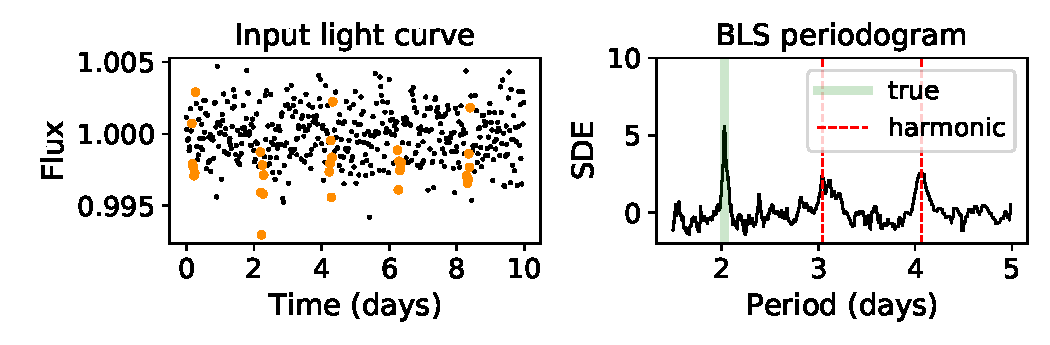
\includegraphics[width=0.7\linewidth]{Background/Figures/BLS_example.pdf}
    \caption{The BLS algorithm applied to the same light curve from Figure \ref{fig:folding}. The highest peak in the periodogram corresponds to the correct period $P$ of the signal. However, the harmonics of the signal, e.g. $3/2P$ and $2P$ as shown here, also produce peaks.}
    \label{fig:bls_example}
\end{figure}

Instead of using the SDE to set a detection threshold, a detection threshold could be set on the signal-to-noise ratio (SNR) of transit candidates. Ignoring the presence of time dependend noise, the SNR can be defined as $\delta / \sigma_w \cdot \sqrt{n_t}$ with $n_t \,\propto\, \tau$ the number of measurements that belong to the transit signal and $\sigma_w$ the estimated white noise in the detrended light curve. However, \cite{pont2006effect} show that a detection threshold for BLS can be set better if time dependend noise is accounted for in the approximation of the SNR. This is likely because background patterns with time scales similar to the transit duration could remain intact after detrending.

Several variants to BLS exist. For example, \cite{carter2013quasiperiodic} relax the assumption of strictly periodic signals, and use a quasi-periodic transit model that is fitted to the data. \cite{foreman2016population} omit the periodicity assumption altogether and use an algorithm similar to BLS to search for monotransits. In their work, a box function is fitted to the data at multiple points in time, and a detection threshold for single events is set on the SNR above the noise floor determined by a sliding median filter.

More recently, the Transit Least Squares (TLS) algorithm was proposed by \cite{hippke2019optimized}. As opposed to BLS, TLS takes into account the effect of limb darkening on the transit shape, and is therefore more expressive than BLS. For this reason, TLS generally performs better at detecting transit signals than BLS, however at the cost of longer computation times.

The performance of BLS and TLS largely depends on the way the light curve is detrended prior to the search. \cite{hippke2019wotan} compare a wide range of detrending methods, before applying TLS to search for transits. They evaluate each method by the extend to which known transit signals are retrieved by the TLS algorithm, after applying the detrending method. The methods evaluated include sliding mean and median filters, Gaussian processes, the Savitzky-Golay filter, and more. The results showed that detrending could significantly alter or reduce the transit signals, for some methods more than others. A time-windowed median filter performed reasonably considering its computational efficiency. Furthermore, for window-based filters, it was found that a window size of three times the transit duration is the best choice for detection. The problem is however, that the presence of a transit is not known beforehand in the task of detection, let aside its duration.

\subsection{Simultaneously modelling background and signal}

In order to avoid the risks that are involved with detrending, one could simultaneously model background stellar activity with the transit signals. This approach was taken by \cite{foreman2015systematic}, where light curves were described as a combination of the 150 most representative components of the principle component analysis (PCA) of K2, while simultaneously fitting for a box-shaped transit model. Since the background is modelled side-to-side with the transit signal, the background model is less prone to overfit to the transit signal, and the transit signal is therefore expected to stay better intact.

In contrast, \cite{kovacs2016periodic} argue that with simultaneous modelling, there are more degrees of freedom and thus more chance of false positives. They found better results by first detrending the light curve, and subsequently searching for transit signals. This approach was also found to be considerably more efficient.

\subsection{Kepler and TESS pipeline}

The pipelines of Kepler and TESS cover the process of reducing raw images of stars to systematics corrected light curves, which are subsequently searched for transit signals. The TESS pipeline is largely based on the Kepler pipeline \citep{jenkins2016tess}, so we base our description of both pipelines on the Transiting Planet Search (TPS) module as described in the Kepler Data Processing Handbook \cite{jenkins2017kepler}. 

In the TPS module, the input light curve first undergoes a series of preprocessing steps, e.g. stitching sectors together and filling data gaps. Subsequently, a time-varying whitening filter is applied, which is supposed to clear the light curve of irrelevant time dependent noise. The use of a pre-whitening filter for transit search has been adopted more often (e.g. \cite{carpano2003detecting}) as it is considered to be the optimal detector in combination with a simple matched filter in the case for colored Gaussian noise, as explained in \cite{jenkins2002impact}. However, \cite{rodenbeck2018revisiting} note that a pre-whitening filter can introduce features that could be misinterpreted as signal. The pipeline therefore removes positive flux outliers which could introduce transit-like features in the whitened flux. Since the whitening filter can also alter transit signals, the same whitening is applied to the transit pulse train that is used as transit model. After single candidate transit events have been identified, a grid of periods, durations and epochs is searched through to find a least squares fit to each potential signal. A representative limb darkening model is used to fit with the data.

Although the pipeline is far in its development and is constantly being improved, it still relies on heavy preprocessing and an extensive search through parameter configurations of potential signals. Furthermore, the TPS module in the pipeline is designed as general algorithm to detect most of the hidden transit signals. Therefore, this algorithm might still miss signals in special cases.

\subsection{Other classical detection methods}

In cases where a periodic signal resembles a sine function, the Fourier transform (FT) provides a good way to detect it. For a transit signal this is in general not the case as its duration is short relative to its period. For ultra-short-period (USP, $< 1$ day) planets on the other hand, the duration becomes larger relative to the period, and the FT will have similar detection performance as the BLS algorithm, as was shown by \cite{sanchis2014study}. In their work, an FT-based detection method is applied to detect transits from USP planets in Kepler data. They argue that the FT produces less disturbing harmonics in its resulting spectrum compared to BLS, but BLS is more effective for longer period planets. 

Another approach to transit detection is to use the dispersion of the phase folded light curve. \cite{plavchan2008near} fold a given light curve over several trial periods, each time evaluating the difference between the folded light curve and its boxcar-smoothed counterpart. A small set of periods for which the folded curve corresponds best to the smoothed phase curve, is further analysed for transits. \cite{wheeler2019weird} also propose a method which aims to minimize the phase dispersion by folding the light curve at different trial periods. Since this method does not assume any specific signal shape, it is sensitive to strictly periodic signals of arbitrary shape. Their method was applied by \cite{chakraborty2020hundreds} to find 377 previously unreported signals in the first year of TESS observations.

\subsection{``Intelligent'' algorithms}

The human eye can function as an excellent tool for pattern recognition and can exceed algorithms in complex ways. For this reason, the citizen science project Planet Hunters was launched. Participants, or users, are presented with light curves from Kepler and asked to flag parts of the light curve that resemble transit signals. Six months after the launch, millions of classifications were made and later \cite{fischer2012planet} reported the detection of the first two planet candidates that were flagged by participating volunteers. This process can also be viewed as a detection algorithm. The user is in this case the detector, which utilizes prior knowledge about the shapes of different transit signals to flag potential signals. Without requiring the light curve to be detrended or folded, individual events are flagged by the detector. If there is enough confidence about a certain signal, i.e. enough users have flagged the same events, the ``detection'' is passed to the vetting stage. For Planet Hunters, this stage consists of experts in the field who rule out clear false positives and conduct follow up observations to confirm the planets. 

Similarly, one could use AI for the task of transit detection. \cite{pearson2018searching} trained a one dimensional CNN to classify light curve segments as signal or non-signal. The CNN lends itself well for identification and forms the basis of several recent works in the field such as \textit{AstroNet} \citep{shallue2018identifying} and variants \citep{ansdell2018scientific, dattilo2019identifying, koning2019reducing, yu2019identifying, osborn2020rapid}. For detection, however, the model is limited by the fact that is only allows relatively small inputs of fixed size. Therefore, \cite{pearson2018searching} propose two approaches to use the CNN for detection. In the first approach, the network is applied to overlapping segments in the light curve to obtain outputs at each point in time, which are referred to as probability time series (PTS). Subsequently, they propose to use the average distance between peaks in the PTS can give an estimate of the periodicity of the signal. In the second approach, the light curve is folded over given trial periods, each time applying the CNN to overlapping segments in the resulting phase curve. A detection in the phase curve directly gives an estimate of the periodicity, but this approach requires the same parts of the light curve to be evaluated many times by the CNN. \cite{zucker2018shallow} tested the feasibility of using CNNs for detection in comparison with the BLS algorithm. Their experiments were based on simulated light curves with Gaussian processes to account for stellar variability. The task they evaluated both methods on was not entirely that of detection, but instead the binary classification task of classifying input light curves as signal or non-signal.

Extending on the work on CNNs, \cite{chintarungruangchai2019detecting} evaluated the use of two-dimensional CNNs for detection. Instead of folding the light curve to one dimension, they fold the light curve such that each folded segment is stacked on top of each other. Subsequently, they train the CNN to classify these two-dimensional ``images'' as signal or non-signal. Although multiple trial periods still need to be evaluated to search for a potential signal, this method is found to be more robust against deviations from the true period than the method proposed by \cite{pearson2018searching}. However, the problem remains that the methods evaluated by \cite{chintarungruangchai2019detecting} and \cite{zucker2018shallow} only provide a binary output for an input light curve, and do not allow to determine the exact timing of the individual signals.

\section{Identification methods}
\red{[TODO]}

\section{Recurrent Neural Network (RNN)}
\red{[TODO]}

\subsection{Application to exoplanets}
In a task that resembles detection, \cite{hinners2018machine} compared a bi-LSTM with a feature engineering approach. Among other tasks, the task was to predict the number of transits present in a given light curve. Their bi-LSTM model produced near-random results. Other tasks included the prediction of parameters of the star given its light curve. They address the problem of the RNN-based model could be due to the fact that their data set was imbalanced. However, we note that it might have been due to the sparse learning signal that is given to the RNN. Namely, only after having seen about 7000 input data points, the RNN receives one learning signal over its single output value. This way, figuring out where transit signals are present in a given light curve can only be implicitly learned by the model, while we can also explicitly provide this information as learning signal at every time step. This idea has motivated us to develop the RNN-based transit detection algorithm presented in this work, which is further described in Chapter \ref{chap:methodology}. 

In another work utilizing LSTMs, \cite{morvan2020detrending} show the successful application of LSTMs for detrending. The model was trained to learn out-of-transit patterns, and interpolate these within the duration of a given transit signal. By doing so, the background signal could be better subtracted from the signal, and thus the transiting planet better characterized. Results improved if centroid data was included.

\subsection{Application to variable stars}
Remaining literature mostly focuses on light curve classification, in general for variable stars. For example, \cite{jamal2020neural} compare different neural network architecture for this task, including dilated temporal convolutional networks (dTCNs), LSTMs, GRUs, temporal convolutional NNs (tCNNs) and encoder-decoder models. The LSTM and tCNN were found to be performing best, with the latter having the benefit of shorter computation times. 

\cite{naul2018recurrent} address the problem of irregularly sampled data in light curves by including time intervals between measurement as input to an RNN encoder. The RNN is used for variable star classification. \cite{becker2020scalable} also experiments with time intervals between measurements as input to the model, and instead of using the raw flux they also use the differences between subsequent flux values as input. To reduce computational requirements, they adopted a sliding window approach over the input light curve, of which each window is used seperately to train the RNN. While most works employ a bidirectional RNN, in this work a unidirectional RNN was used to allow for its application in an online fashion.

% \cite{tsang2019deep} jointly train an RNN with an autoenconder to reconstruct and classify variable star light curves. They use a Gaussian mixture model to detect novel light curves.

\subsection{Anomaly detection}
Transit signals can be seen as anomalies in time series of ``normal'' stellar behaviour. LSTMs have been used to detect anomalies in time series in an unsupervised learning approach by \cite{malhotra2015long}. In this case, the LSTM is trained to predict the normal data and the errors on the predictions are used to threshold the detection of an anomalous event. If the LSTM is trained to predict multiple steps into the future, the same approach can be used to detect collective anomalies \citep{bontemps2016collective}, for example transit signals which generally cover multiple data points. However, as \cite{cherdo2020training} noted, this `unsupervised' approach to using LSTMs for anomaly detection still requires training on normal data, i.e. we need to know beforehand which data is clear of anomalous events. In our case, we might never be fully sure to whether a light curve is clear of transit signals, e.g. small and previously unseen signals might still be hidden in the data. Training the model to treat these light curves as ``normal'' data, might seriously harm the ability of the model to detect the smallest transit signals. For our purposes, we therefore turn to the supervised approach, as we can utilize both the transit signals from known exoplanets as well as realistically simulated signals as inputs to our model. 

\subsection{Irregularly-sampled time series}
Although attempts have been made to handle irregularly sampled time series using RNNs for variable star classificiation, developments within AI can provide different perspectives on the problem. Not related to variable stars but related to handling irregular time series using RNNs, is the ODE-RNN \cite{rubanova2019latent}. This model design, inspired by \cite{chen2018neural}, treats time as continuous, whereas the standard RNN treats time as discrete steps. The ODE-RNN can handle arbitrary time gaps between observations, which could be useful for our purposes. However, this comes at the cost of a required altering of the training process as opposed to using a standard RNN, in which batched training does not come straightforward. Moreover, the benefits of the ODE-RNN are most profound if the sampled data is sparse. With transit durations in the order of hours and a observation cadence in the order of minutes, this is generally not the case. For this reason, we rely on the standard RNN architectures in this work, and leave the application of ODE-RNNs for exoplanet science for future work.

\section{Other relevant work in AI}
\red{[TODO]}

\subsection{Uncertainty in neural networks}
Although the topic of uncertainty can be a thesis subject on its own, we briefly touch on the subject as uncertainties could play a role in the task of transit detection. For example, if multiple candidate transit signals are detected and detector's response is similar for all, we might wish to accept only the signals for which the detection uncertainty is below a certain threshold. For neural networks, though in some cases their output has some probabilistic meaning, in general one must be cautious with interpreting their outputs as probability. If unseen out-of-distribution data is presented to the network, which differs substantially from the training data, its outputs might not make sense anymore. \red{[TODO: explain: why would out of dist data occur?]} Instead, it would be convenient if the network outputs an additional value that indicates the confidence of a certain classification. 

\cite{gal2016dropout} describe how dropout with repeated application of the network can be used to obtain uncertainty estimates over predictions. Although this approach is appealingly simple, a few problems remain. First of all, this approach might not solve the problem, because for each instance of the model the data would remain out-of-distribution, and might trigger an erroneous detection in each case with low uncertainty as a result. Furthermore, as RNNs are already less efficient than for example CNNs, the need for repeated application might harm their scalability considerably. Obtaining reliable uncertainty estimates for RNNs is not a straightforward task. Work on uncertainty estimation for RNNs is still being published \citep{alaa2020frequentist, hwang2020sampling, wang2020uncertainty}. For our purposes, we use the method proposed by \cite{devries2018learning} and explore it for our task. Their approach is to adjust the loss function that is used for training, such that the network learns for which inputs it is more certain of its outputs and vice versa. The details and integration of this method in combination with our RNN is described in Chapter \ref{chap:methodology}.

% \cite{le2020contrastive} describes the contrastive learning framework.

% \cite{he2009learning} describe ways to deal with imbalanced data sets.

% Exploding gradients in GRUs are known to be a problem \cite{kanai2017preventing}.

\chapter{Methodology}
\label{chap:methodology}

Since this work makes use of simulated light curves, the following sections describe in detail how the data was obtained that was used. Subsequently, the network design and training procedure are described as well as the extensions that were explored. Baselines and specific parameter choices which are dependent on the experiments, are described in the corresponding sections in Chapter \ref{chap:experiments}.


\section{Data simulations}

For the development and evaluation of our RNN-based algorithm we used simulated data. This is because simulated data comes with an absolute ground-truth of the hidden signals, and for the development of the algorithm it showed useful to be in control over the parameters of the input light curves. In contrast, real-world data cannot be changed, and in some cases the ground-truth is ambiguous. Realizing that a single source of simulated data may limit our results, two sources of data were used. First, our Light Curve Simulator, or LCSim, was specifically designed for this work. Second, we made use of simulated light curves in the Lilith-4 data set, which was produced by the Lilith data simulator of the TESS pipeline. The following subsections describe the details of the simulations, the data sets used in this work, and some general preprocessing of the data.

\subsection{LCSim}
\label{sec:lcsim}

In line with TESS data, we adopt a 2-minute cadence for all simulations in this work. The simulator, made available here\footnote{\url{https://github.com/ykerus/transit-detection-rnn15}}, may also be used to generate 30-minute cadence light curves, to obtain light curves that are closer to Kepler data. 

Stellar variability is simulated using Gaussian processes (GPs). GPs have been used several times in literature to account for background activity in light curves, both for characterizing and simulating stellar activity \citep{barros2020improving, zucker2018shallow}. GPs are defined by a mean and a covariance function, or kernel. In our case, the mean function is always 1, so the behaviour is fully determined by the kernel, which should therefore hold all of the star's relevant properties. An instance of the function representing stellar variability can be obtained by sampling from the multi-dimensional Gaussian distribution that is defined by the mean and covariance function. However, if we use the same kernel for each sample, then each light curve has the same underlying stellar properties. Therefore, we construct a kernel for each light curve. To construct a kernel that is able to simulate quasi-periodic behaviour as observed in stars, we make use of the Python library \texttt{celerite} \citep{foreman2017fast}. \todo{cite use cases of celerite} \texttt{celerite} has built-in kernels to simulate stellar granulation and rotation modulation. These kernels are specified by the standard deviations and time scales of the processes, among several other parameters which are given in Table \ref{tab:params}. The two oscillation terms describing stellar rotation are partly defined by $Q_0$, $\text{d}Q$ and $f$ which respectively describe the quality factor of the secondary oscillation, the difference between quality factors of both oscillation modes, and the fractional amplitude of the secondary mode compared to the primary (see the documentation\footnote{\url{https://celerite2.readthedocs.io/en/latest/api/python/}}). $P_{\text{rot}}$ and $\sigma_{rot}$ describe the primary period of the rotation and the standard deviation of the variability respectively. For the granulation term, we have $P_\text{gran}$ and $\sigma_\text{gran}$ to describe the period and standard deviation, and $Q$ the quality factor of the oscillation. For granulation it is standard to choose $Q=1/\sqrt{2}$ \todo{cite}.

To simulate photon noise, we sample from a Gaussian distribution $\epsilon_{ij} \sim \mathcal{N}(0, \sigma_i)$ and add $\epsilon_{ij}$ to the corresponding flux at time step $j$ in light curve $i$. The standard deviation $\sigma_i$ ($\sigma$ in Table \ref{tab:params}) defines the level of time-independent noise in the light curve, and is specified for each light curve separately. 

For the simulation of transit signals, we made use of the Python library \texttt{batman} \citep{kreidberg2015batman}, which is based on the equations from \cite{mandel2002analytic} which describe the physics of transits. We approximate the stellar limb darkening effect with the built-in quadratic function, parametrized by $u_1$ and $u_2$. The values for these parameters were sampled using intermediate parameters $q_1$ and $q_2$ such that they always produce physical transit signals, according to \cite{kipping2013efficient}. We constrained the orbital period $P$ of a planet and its semi-major axis $a$ according to Kepler's Third Law (see Section \ref{sec:transit}). In order to do so, we also specify the stellar mass $M$ and radius $R$ so the result is compatible with the input requirements of \texttt{batman}. The orbital inclination $i$ is assumed to be 90$^\circ$ for all planets we simulate, to avoid problems with non-existent transit signals, or transit depths that are more difficult to predict. Setting $i=90^\circ$ ensures that a simulated planet moves in front of the stellar disk during transit. The eccentricity $ecc$ is sampled from a Beta distribution, following \cite{kipping2013parametrizing}. The radius of the planet is specified by $ror$, which is fractional radius of the planet relative to its host star. Lastly, $w$ is specified to indicate in which part the exoplanet is in its orbit when it transits its host star. If $ecc=0$, then $w$ has no effect, otherwise $w=90^\circ$ will correspond to the shortest possible transit duration, and $w=270^\circ$ to the longest.

In case a light curve is required to have transit signals from multiple different planets, the transit simulator is simply called iteratively with different parameters for the planets while maintaining all the parameters belonging to the star. The result might be that the two planets coincidentally have the same distance from their host star, which would be unrealistic, but does not pose a problem for the purpose of this thesis. Overlapping transit signals, on the other hand, could make the process of developing and evaluating our detection algorithm more difficult. If overlapping signals have been found, one needs to make sure which signal triggered a detection: it could be one of the two, or both. Since overlapping signals are far less common in real-world data than non-overlapping signals, we only simulate non-overlapping transit signals in this work to avoid confusion.

Several data sets used in this work are based on LCSim. LCSim-1500 is a set of light curve segments consisting of $N=1500$ data points per light curve, which is used for training and evaluating the network. These light curves are supposed to imitate light curve segments that are obtained from splitting an original full-length light curve into parts. However, with LCSim we simulated the segments directly to reduce computational costs, so we do not have access to the ``original'' light curves. LCSim-500 is similar, only it has fewer ($N=500$) data points per light curve. Both data sets contain 15000 training samples, 5000 validation samples and 5000 test samples. Half of the samples per split contains no transit signals, 35\% contains a single transit signal and 15\% two transit signals. For the evaluation of our method's ability to retrieve signals in full-length light curves, we use LCSim-Mono and LCSim-Single. Both data sets consist of 5000 light curves spanning 27.4 days (i.e. 19728 data points per light curve). 50\% of the samples in LCSim-Mono contain a single transit signal, and 50\% of the samples in LCSim-Single contain at least three transit signals from a single transiting planet. None of these data sets contain data gaps. However, to evaluate the effect of gaps and different gap-handling approaches, we use LCSim-1500-Gap, which is LCSim-1500 with injected gaps. Zero, one or two large gaps between 2 and 10 hours are injected with 50\%, 35\% and 15\% probability respectively. In addition, a random selection of 2\% of the data points is removed. For the training of the representation RNN, we generated pairs of white-noise dominated light curves with the same distribution of transit signals as for the other data sets. 50\% of the samples was a positive pair, and 50\% a negative pair, as explained in \ref{sec:rnn_repr}.

Each light curve is directly simulated as median normalized, i.e. centered around 1. Prior to applying the RNN, we always center the inputs around zero by subtracting 1, and standardize the entire data set. To do so, for each data point we subtract the mean and divide by the standard deviation over all data points in the training split. In Chapter \ref{chap:experiments}, we experiment with additional preprocessing steps.

%\cdashlinelr{1-4}


\begin{table}[]
\centering
\begin{tabular}{@{}llll@{}}
\toprule
                      &  Parameter               & Sampling distribution or relation                           & Units            \\ \midrule
Photon noise          & $\sigma$        & $\exp(\text{Uniform}(\log(0.0005), \log(0.003)))$           & -                \\ \cdashlinelr{1-4}
\multirow{5}{*}{\begin{tabular}[c]{@{}l@{}}Stellar\\ rotation\end{tabular}} &
  $Q_0$ &
  $\text{LogNormal}(0, 2)$ &
  - \\
                      & d$Q$            & $\text{LogNormal}(0, 2)$                                    & -                \\
                      & $f$             & $\text{Uniform}(0.1, 1)$                                    & -                \\
                      & $P_{rot}$       & $|\text{Normal}(5,2)| + 1$                                  & days             \\
                      & $\sigma_{rot}$  & $\exp(\text{Uniform}(\log(0.0003), \log(0.005)))$           & -                \\\cdashlinelr{1-4}
\multirow{4}{*}{\begin{tabular}[c]{@{}l@{}}Stellar \\ granulation\end{tabular}} &
  $\nu$ &
  $\text{LogNormal}(4.5,1) \cdot 10^{6}$ &
  Hz \\
                      & $P_{gran}$      & $1/\nu/86400$                                               & days             \\
                      & $\sigma_{gran}$ & $\text{LogNormal}(\log(\num{2e-6} \cdot \nu^{-0.61}), 0.1)$ & -                \\
                      & $Q$             & $1/\sqrt{2}$                                                & -                \\ \cdashlinelr{1-4}
\multirow{5}{*}{Star} & $M$             & $|\text{Normal}(0.9, 0.25)| + 0.1$                          & $\text{M}_\odot$ \\
                      & $R$             & $|\text{Normal}(M^{1/3}-0.1, 0.2)| + 0.1$                   & $\text{R}_\odot$ \\
                      & $q_1$, $q_2$    & $\text{Uniform}(0, 1)$                                      & -                \\
                      & $u_1$           & $2 q_2\sqrt{q_1}$                       & -                \\
                      & $u_2$           & $(1-2q_2)\sqrt{q_1}$                                        & -                \\\cdashlinelr{1-4}
\multirow{5}{*}{Exoplanet} &
  $P$ &
  $\exp(\text{Uniform}(\log(P_{min}), \log(P_{max})))$ &
  days \\
 &
  $a$ &
  $( (M \cdot \text{M}_\odot)\cdot 86400P \cdot G / (2\pi)^2 )^{1/3} / (R\cdot\text{R}_\odot)$ &
  $R$ \\
                      & $ror$           & $\exp(\text{Uniform}(\log(0.02), \log(0.15)))$              & -                \\
                      & $ecc$           & $\text{Beta}(0.867, 3.03)$                                  & -                \\
                      & $i$             & $90$                                                        & deg              \\
                      & $w$             & $\text{Uniform}(0, 360)$                                    & deg              \\ \bottomrule
\end{tabular}
\label{tab:params}
\caption{Sampling distributions for the parameters used in LCSim (see main text for their descriptions). Inspiration for these distributions came from online tutorials, e.g. from \texttt{exoplanet} \citep{exoplanet:joss} for  $Q_0$, d$Q$ and $f$; literature, e.g. \cite{martins2020search} for stellar rotation, \cite{kallinger2014connection} for granulation, \cite{kipping2013efficient} and
\cite{kipping2013parametrizing} for efficient sampling of $ecc$, $u_1$ and $u_2$; and parameter values from known transiting planets and real-world light curves from TESS \citep{ricker2014transiting} for remaining planetary and stellar parameters and photon noise. $\text{M}_\odot = \num{1.989e30}$ kg and $\text{R}_\odot = \num{6.963e8}$ m are the solar mass and radius, $G$ is the gravitational constant, and $P_{\text{min}}$ and $P_{\text{max}}$ a pre-defined minimum and maximum orbital period of the planet. Note that the relations between parameters are in some cases not realistic. For example, $M$ and $R$ are only sampled to get a reasonable and slightly random relation between $P$ and $a$, but themselves have no other function in the simulation. However, for the purpose of our research this is no problem as we do not make explicit use of these parameters in our detection algorithm, and the transit signals are still defined by a complex interplay between the parameters specified above.}
\end{table}


\subsection{Lilith-4}
\label{sec:lilith-4}

The Lilith-4 data set comprises four sectors of simulated TESS data, and takes into account readout errors, spacecraft jitter, focus errors, diffuse light, cosmic rays, stellar variability, transiting exoplanets, eclipsing binary stars, and more \citep{smith2019four}. This simulated data set is therefore expected to be considerably more realistic than ours, which is why we include it in this research.   Furthermore, it allows for the evaluation of certain preprocessing steps in combination with our algorithm, that would be necessary in the case of using real-world data. Lilith-4 also includes information about the pointing of the telescope, the centroid data, which can be used by our algorithm to potentially benefit from.

We prepared two data sets based on Lilith-4. As explained in Section \ref{sec:astro_false_pos}, we excluded light curves with (B)EB signals. The first data set, Lilith-1500, is similar to LCSim-1500. Lilith-1500 is obtained from median normalizing the light curves that only span a single sector in Lilith-4, and subsequently splitting them into equally sized segments of $N=1500$ data points. Missing data points are replaced with NaN values, and slight deviations from a 2-minute cadence are corrected for. The segments were chosen to be partially overlapping, so we have more data to train the network. Segments are rejected if they contain transit signals which are less than half visible, overlapping, less than 1 or more than 13 hours in duration, or have a depth $\delta$ relative to $\sigma$ (i.e. $\delta/\sigma$) of less than 0.25 or more than 10. For Lilith light curves, $\sigma$  is not given, so we estimate it by flattening the input with a sliding median filter with a window size of 30 minutes, and subsequently taking the standard deviation. From a total of 68236 segments, 61\% was used for training, 22\% for validation and 17\% for testing. Segments from the same light curve were kept in the same split, to avoid overlap between training and test data. To evaluate the ability of our algorithm to detect planets in Lilith light curves, we prepared Lilith-Multi. This data set consists of 6511 light curves which were excluded from Lilith-1500, 2670 of which contained at least three transit signals from at least one planet. We used light curves of each sector separately, so we did not stitch light curves from targets which had observations over multiple sectors. Only planets with at least three transit signals in the same light curve with relative transit depths $0.25 < \delta/\sigma < 10$ were used in the evaluation. Regarding preprocessing, we take the same steps as for LCSim data. Additionally, we filtered out flagged low-quality data points, using the flags explained by \cite{tenenbaum2018tess}.



\section{Network}
\label{sec:network}

The basis network architecture, training objective and procedure are described in the following sections. The main task of the network is to classify individual data points as signal or non-signal, where every data point within the duration of a transit is considered as part of the signal. Extensions, such as the prediction of flux values within data gaps, are described in separate sections, as these require slightly different network architectures and training. A visualization of the network is given in Figure \ref{fig:network}. All of the following was implemented using PyTorch (version 1.8.1). 

\begin{figure}
    \centering
    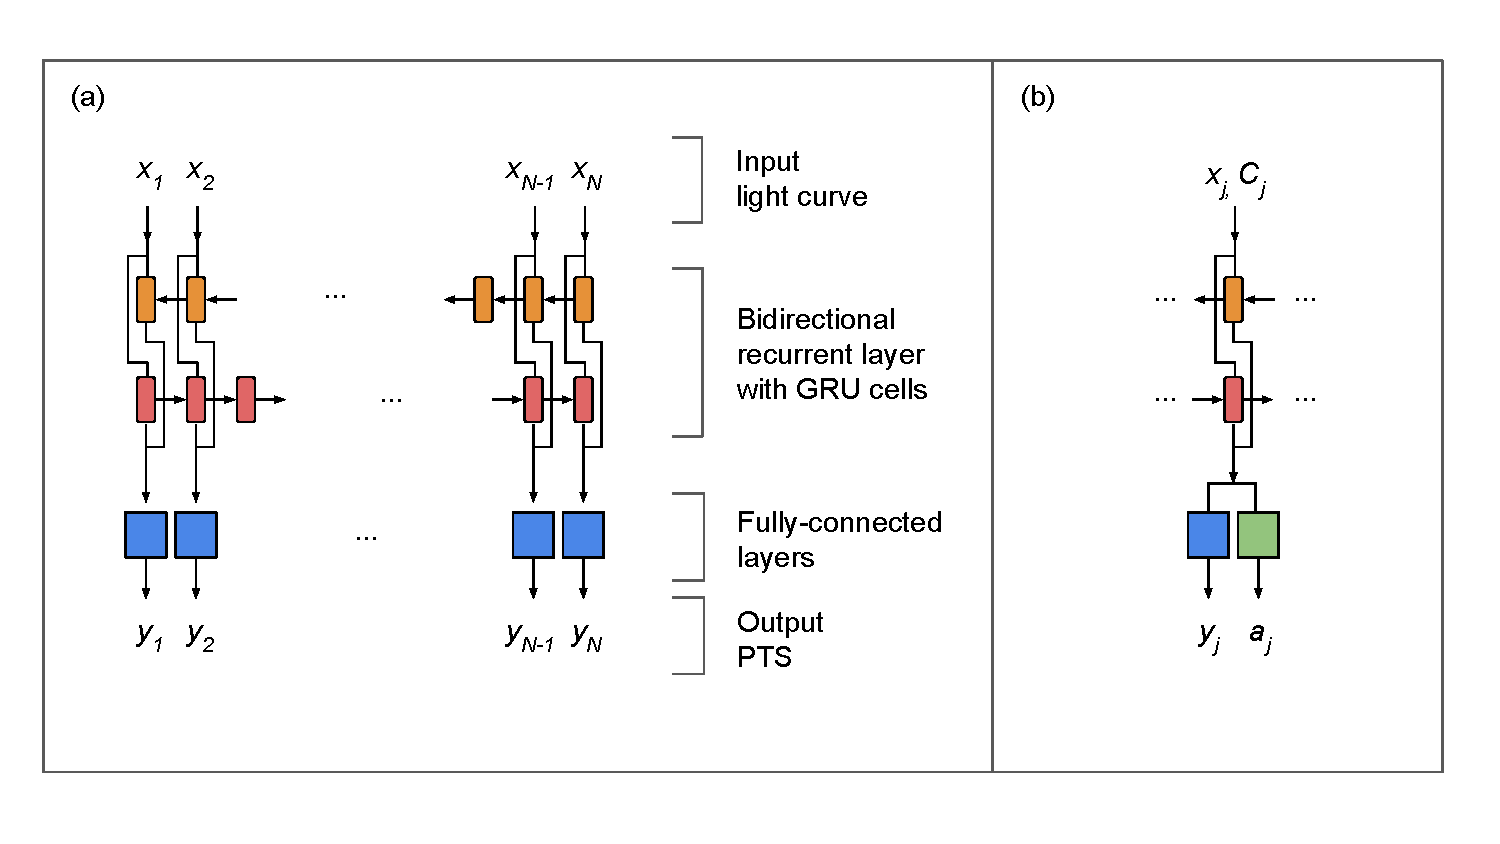
\includegraphics[width=0.7\linewidth]{Methodology/Figures/network_drawing.pdf}
    \caption{(a) The basis RNN which takes as input $x_1,\dots,x_{N}$ and outputs $y_1,\dots,y_{N}$. Colors indicate which blocks share the same weights and arrows indicate the flow of information. The outputs of both components of the bidirectional recurrent layer are concatenated before they are passed to the fully-connected (FC) layers. (b) The network is extended in several ways. First, we may use additional inputs $C_j$, e.g. centroid data, at each time step $j$. Second, we may add an additional network of FC-layers, to obtain an additional outputs $a_j$, e.g. confidence values, or representation vectors. }
    \label{fig:my_label}
\end{figure}

\subsection{Architecture}
\label{sec:architecture}

Since light curves may contain thousands of data points, we avoid the ``vanilla''-RNN, which is known to suffer from vanishing gradients. Other recurrent cells considered were GRU and LSTM. We found GRU to produce better and more stable results than LSTM, which is why we used GRU in our basis RNN design. Both directions in time are relevant for the classification of a data point. For example, both ingress and egress are strong features of a transit signal. This means that at mid-transit, knowing information from both directions could make it easier to classify the data points, compared to only knowing the past. For this reason, we make use of a bidirectional RNN, i.e. bi-GRU.

In order to classify each time step as signal or non-signal, the output of the network should be a single value at each time step. To achieve this, we apply fully connected (FC) layers to the outputs of the recurrent layers, which project the hidden representation at each time step down to a single node. The result is passed through the sigmoid activation function, so the outputs lie between 0 and 1. Between fully connected layers, the ReLU activation function is applied to introduce non-linearities. For most experiments, we used a bi-GRU with a single recurrent layer consisting of 64 hidden nodes, and two fully connected layers, both consisting of 64 nodes. This network was obtained by informal hyperparameter tuning, and comparison against different architectures (see Section \ref{sec:models}).

\subsection{Training}
\label{sec:training}

In a supervised fashion, we train the network to classify data points as signal or non-signal. This requires knowing the ground truth of the data. In our case we use simulated data, so we have access to the ground truth. Alternatively, one could use known (non-)transit signals in real-world light curves as ground-truth, or inject simulated transit signals in real-world light curves. 

Typical light curves, however, contain too many data points to be used for training directly. First of all, the training procedure requires storing the gradients at each time step which would quickly overflow memory. Second of all, the RNN cannot well learn dependencies over thousands of time steps, because even LSTM and GRU have forget and reset gates, so using full-length light curves for training would be unnecessarily inefficient. Therefore we assume that the data used for training consists of light curve segments, obtained by splitting the original light curve in segments of equal length $N$. $N$ should be chosen larger than the typical transit duration ($\sim$6 hours) so sufficient background activity is included in the segments, but small enough to allow for efficient training. This work uses $N=1500$ for the training of the network, which corresponds to 50 hours for a cadence of 2 minutes, unless stated otherwise.


The network is used to model $p(T|X)$, where $T$ represents the targets $\{t_j\}_{j=1}^N$ for each data point $\{x_j\}_{j=1}^N$ in a given light curve segment $X$. We assume the network inputs to be preprocessed such that the flux values $x_j$ can take any value, i.e. $x_j \in \mathbb{R}$. A target $t_j$ is 1 if $x_j$ is part of a transit signal, otherwise it is 0. We assume that the target $t_j$ depends on all flux values through $x_j$, which is dependent on its neighbours $x_{j\pm1}$, which are dependent on their neighbours, and so on. This can be visualized by:

\begin{figure}[H]
\centering
  \tikz{
% nodes
%  \node[obs]
 \node (xa) {$\dots$};%
 \node[obs,right=of xa] (xb) {$x_{j-1}$};%
 \node[obs,right=of xb] (xc) {$x_{j}$};
 \node[obs,right=of xc] (xd) {$x_{j+1}$};
 \node[right=of xd] (xe) {$\dots$};%
 
 \node[latent,below=of xb] (tb) {$t_{j-1}$};
 \node[latent,below=of xc] (tc) {$t_{j}$};
 \node[latent,below=of xd] (td) {$t_{j+1}$};

\edge [-] {xb} {xa, xc};
\edge [-] {xd} {xc, xe};
\edge {xb} {tb};
\edge {xc} {tc};
\edge {xd} {td};
  }
\end{figure}
\noindent Since we observe $X$, the targets become separated in the graphical model. Therefore we model them as independent, given $X$, i.e.:
\begin{equation}
    p(T|X) = p(t_1,\dots,t_N|X) = \prod_{j=1}^N p(t_j|X)
\end{equation}
In other words, we assume that knowing the a target $t_{k}$ at time step $k \neq j$ in addition to the flux values $X$, would not make a difference for the probability of observing $t_j = 1$, compared to only knowing $X$. Therefore, the only information we feed to the network at each time step is $x_j$.

Our network outputs a value $y_j \in (0,1)$ for each $x_j$, using the function $Y = f(X, W)$, where $W$ represents the weights of the network. $Y$ represents the collection of outputs $\{y_j\}_{j=1}^N$. We interpret $y_j$ as the conditional probability $y_j = p(t_j=1|X,W)$, such that $p(t_j=0|X,W)$ is given by $1-y_j$. The conditional distribution of targets at time step $j$ is then given by:
\begin{equation}
    p(t_j|X,W) = y_j^{t_j} (1-y_j)^{1-t_j}
\end{equation}

\noindent Given a set of independent observations $\{T_i\}_{i=1}^M$ for light curve segments $\{X_i\}_{i=1}^M$, we aim to maximize the likelihood $p(T|X,W)$ by updating the weights $W$ of the network. Equivalently, we can maximize the log likelihood, which is given by:
\begin{align}
    \log p(T|X,W) &= \sum_{i=1}^M \log  p(T_i|X_i,W) \\
    &= \sum_{i=1}^M \log \prod_{j=1}^N p(t_{ij}|X_i,W) \\
    &= \sum_{i=1}^M \sum_{j=1}^N \log [ y_{ij}^{t_{ij}} (1-y_{ij})^{1-t_{ij}} ] \\
    &= \sum_{i=1}^M \sum_{j=1}^N t_{ij} \log y_{ij} + (1-t_{ij}) \log(1-y_{ij}),
\end{align}

\noindent where $t_{ij}$ represents the target at time step $j$ in light curve $i$ and $y_{ij} = y(X_i,W)_j$.

To define our loss function, which we aim to minimize, we take the negative of $\log p(T|X,W)$, averaged over the number of samples $M$ and the number of data points per sample $N$, i.e. for a single light curve segment $i$ we have the loss:
\begin{equation}
    \mathcal{L}_{\text{BCE},i} = \frac{1}{N}\sum^{N}_{j=1} l_{ij} + (1 - t_{ij}) \log (1 - y_{ij}),
\end{equation}

\noindent where we used $l_{ij} = t_{ij} \log( y_{ij})$, and the subscript BCE because this is known as the binary cross-entropy loss.
Using this loss function for a batched training with $M$ light curve segments per batch, we get:
\begin{equation}
    \mathcal{L}_{\text{BCE}} = \frac{1}{M} \sum_{i=1}^M \mathcal{L}_{\text{BCE},i}.
\end{equation}



In terms of individual data points, however, we are dealing with a highly unbalanced data set, because there are many more non-signal points than signal points. In order to deal with unbalances, we use a different definition of $l_{ij}$:

\begin{equation}
    l_{ij} = p_t w_{ij} t_{ij} \log( y_{ij} ).
\end{equation}

\todo{references of loss weighting}
Here $p_t$ is the positive weight, which is used to tune the weight of positive samples, i.e. the data points which are part of a transit signal. If $p_t > 1$, then the predictions over signal data points will be given extra weight in the loss function. For a given classification threshold, increasing $p_t$ will increase the recall, but will also lower the precision. In addition to the weight $p_t$, which is the same for all positive samples, we explore the use of transit-specific weighting. It might be that the data set contains more shallow than deep transit signals, in which case we may choose to increase the weight of data points belonging to deep transit signals in the data set, and vice versa. This can be done by letting the weight $w_{ij}$ depend on the depth $\delta_{ij}$ of the transit signal at time step $j$. For example, we can set $w_{ij} = \delta_{ij} / \sigma_{i}$, where $\sigma_i$ is the estimated level of white noise in light curve $i$, so $w_{ij}$ depends on the relative transit depth rather than absolute transit depth. In this case, predictions over data points belonging to a transit signal which is twice as deep as another signal in the same light curve, will get twice the weight in the loss function. In case both $p_t$ and $w_{ij}$ are used, a small adjustment to $p_t$ needs to be made for maintaining consistent results between different choices for $w_{ij}$. The new weight for signal data points during training becomes  $p_t' = p_t \cdot \sum_{ij} t_{ij} / \sum_{ij} w_{ij}$, where for $w_{ij} = t_{ij}$ we have $p_t' = p_t$.

Finally, we found that applying weight decay helped to prevent exploding gradients in the GRU. Simply clipping gradients above a certain value would sometimes fail when gradients jumped to infinity in a single training step, causing the training stop before they could be clipped. Weight decay is used as implemented in PyTorch, i.e. decoupled weight decay from \cite{loshchilov2017decoupled}. A weight decay with tuning parameter $\alpha=\num{5e-5}$ was sufficient in most cases.



\section{Detection algorithm}
\label{sec:algorithm}

In case the search for signals is directed towards monotransits, the network outputs for a given input light curve can directly be used for detection. For example, one can set a threshold on peaks in the PTS, which can be considered as candidate detections. In case we wish to search for repeating signals, the RNN outputs alone are not enough. In order to compare the performance of an RNN-based detection algorithm with conventional methods such as BLS, we also need to determine the period and epoch of the signal. Two different algorithms are tested to do so, which only make use of the RNN outputs, i.e. the PTS, for a given input light curve. 

\subsection{PTS-Peak}
\label{sec:pts-peak}
As proposed by \cite{pearson2018searching}, one could use the distances between peaks in the PTS to determine the period of a repeating signal. Here we implement this idea and refer to the algorithm as PTS-Peak. In order for this algorithm to work well, we need to take into account the presence of potential false detections in the PTS, or multiple detections of signals belonging to different planets. Therefore we adopt several rules and filtering steps to ensure consistency between matched peaks and resulting parameter estimates. The algorithm we used takes the following steps:

\begin{enumerate}
    \item The PTS is smoothed using a one-dimensional Gaussian filter with a standard deviation of 9 data points, and peaks above a pre-set threshold are identified and indexed.
    \item For each peak $i$, the width of the peak above the threshold is used as candidate transit duration $\tau_i$ and the central point of the peak as candidate mid-transit time $t_{\text{mid},i}$. For each pair of peaks \{$i$, $j$\}, where $j>i$, the candidate period is determined by $P_{i,j} = t_{\text{mid},j} - t_{\text{mid},i}$.
    \item  For each pair of peaks \{$i$, $j$\}, a set is $c$ formed consisting of the indices of peaks that may correspond to signals from the same planet. The peak $k$ that has $t_{\text{mid},k}$ closest to time $t_{\text{exp}} = t_{\text{mid},j} + P_{i,j}$ is added to the candidate signal set $c=$ \{$i$, $j$\}, if $t_{\text{mid},k}$ is within three hours of $t_{\text{exp}}$. We then get the candidate $c=$ \{$i$, $j$, $k$\}, which is used to update the expected period, i.e. $P_{i,j,k} = (t_{\text{mid},k} - t_{\text{mid},i})/2$. Iteratively, the candidate set is expanded with the indices of peaks that lie within the expected range, until $t_{\text{exp}} - 3\text{h}$  is larger than the maximum time in the PTS. Candidate sets that have missing peaks at times where you would expect them are rejected and the rest is passed to the next step. Note that this would filter out detections if only a single peak is missing in the PTS. However, such signals can still be retrieved by evaluating the harmonics of a detected signal, as is described in step \ref{step:harmonics}.
    \item For each candidate $c$, the candidate duration $\tau_c$ is defined by the median duration of the individual peaks, the period $P_c$ by the median distance between peaks and the $t_{0,c}$ by the median of the epoch expected from subtracting $P_c$ from each individual $t_{\text{mid},i}$. A candidate is rejected if $\tau_c$ is smaller than 15 minutes or if $P_c < P_{\text{min}}$ for a pre-set minimum period $P_{\text{min}}$.
    \item\label{step:score} Each candidate is then given a score. For each individual event $n = \{0,\dots,E-1\}$ in the candidate signal defined by $t_{0,c}$, $\tau_c$ and $P_c$, i.e. $t_{0,c} + nP_c - \frac{1}{2}\tau_c< t < t_{0,c} + nP_c + \frac{1}{2}\tau_c$, the maximum in the PTS is recorded as $y_{n,\text{max}}$. The candidate score is then given by:
    \begin{equation}
        score = \frac{1}{\sqrt{E}}\sum_{n=0}^{E-1} y_{n,\text{max}},
    \end{equation}
    where the square root is used to prioritize detections with more individual events over detections with similar scores $y_{n,\text{max}}$, but fewer events. Only the best scoring candidate is passed to the next step.
    \item\label{step:harmonics}  Finally, the harmonics of the candidate signal are evaluated to allow signals to be detected which have missing peaks in the PTS. For each harmonic $h=\{2,3,\dots\}$, the score is determined similarly to step \ref{step:score}, but with $P_c/h$ and corresponding epoch $t_{0,h}$ instead of $P_c$ and $t_{0,c}$. $h$ is iteratively increased until $P_c/h < P_{\text{min}}$.  The best score and the corresponding parameters are passed to the next step.
    \item To search for multiple planets in a single light curve, the events from the best scoring candidate are masked in the PTS and the process is repeated. The best score and corresponding parameters after each iteration are returned as potential detection. The score is used to set a detection threshold.
    
    
\end{enumerate}
 
\subsection{PTS-Fold}
\label{sec:pts-fold}

It could be that individual transit events are missed by the RNN, or that peaks in the PTS are too weak to be taken into account by PTS-Peak. To be less dependent on distinguishable peaks in the PTS, but more on overall response to transit signals, we define another algorithm which we refer to as PTS-Fold. This algorithm is similar to many existing detection algorithms (e.g. phase dispersion minimization or BLS) in that it folds the input time series over a set of trial periods. However, whereas other algorithms fold the raw light curve over trial periods, PTS-Fold only folds the PTS. Since each value the PTS indicates the extend to which a transit signal might be present at the corresponding time step, we can efficiently compute a candidate detection score for repeating signals by aggregating overlapping data points in the folded PTS. To clarify, the algorithm used takes the following steps:

\begin{enumerate}
    \item The PTS is smoothed using a one-dimensional Gaussian filter with a standard deviation of 9 data points.
    \item A set of trial periods is determined based on the time steps in the PTS. Our input is of 2-minute cadence, so the trial periods are exactly multiples of 2 minutes. The differences between subsequent trial periods increases roughly linearly with the value for the trial period to reduce computational requirements.
    \item For each trial period, the PTS is folded such that at each point in the phase curve consists of a set of overlapping points. 
    \item For each fold, each point in the phase curve is given a score by aggregating the individual overlapping PTS values, i.e. for a single point with overlapping values $y_0,\dots,y_{E-1}$:
    \begin{equation}
        score = \frac{1}{\sqrt{E}} \sum_{n=0}^{E-1}y_n.
    \end{equation}
    The maximum scoring point and corresponding value for epoch for each fold is passed to the next step. 
    \item The result, i.e. the maximum score for each trial period, defines the PTS-Peak periodogram and can directly be used to set a detection threshold. For example, a peak in the periodogram above a given threshold may indicate a detection with corresponding parameters for the period and the epoch.
    \item To search for multiple planets in a single light curve, we mask the previously detected signal in the PTS and repeat the process. However, in order to mask detected signals, we need to have an estimate of the duration of the individual events. For efficiency, we avoided the determination of the duration during search. To obtain a rough estimation for the duration but maintain this efficiency, we therefore use the width $\Delta P$ of the peak in the periodogram at half of its maximum, and translate this to the candidate duration according to $\tau_c = (E-1)\frac{1}{2}\Delta P$, where $E$ is the number of events belonging to the detected signal. The relation between the peak width and the duration of the signal is illustrated in Figure \ref{fig:fold_drawing}.
    
    
\end{enumerate}


\begin{figure}
    \centering
    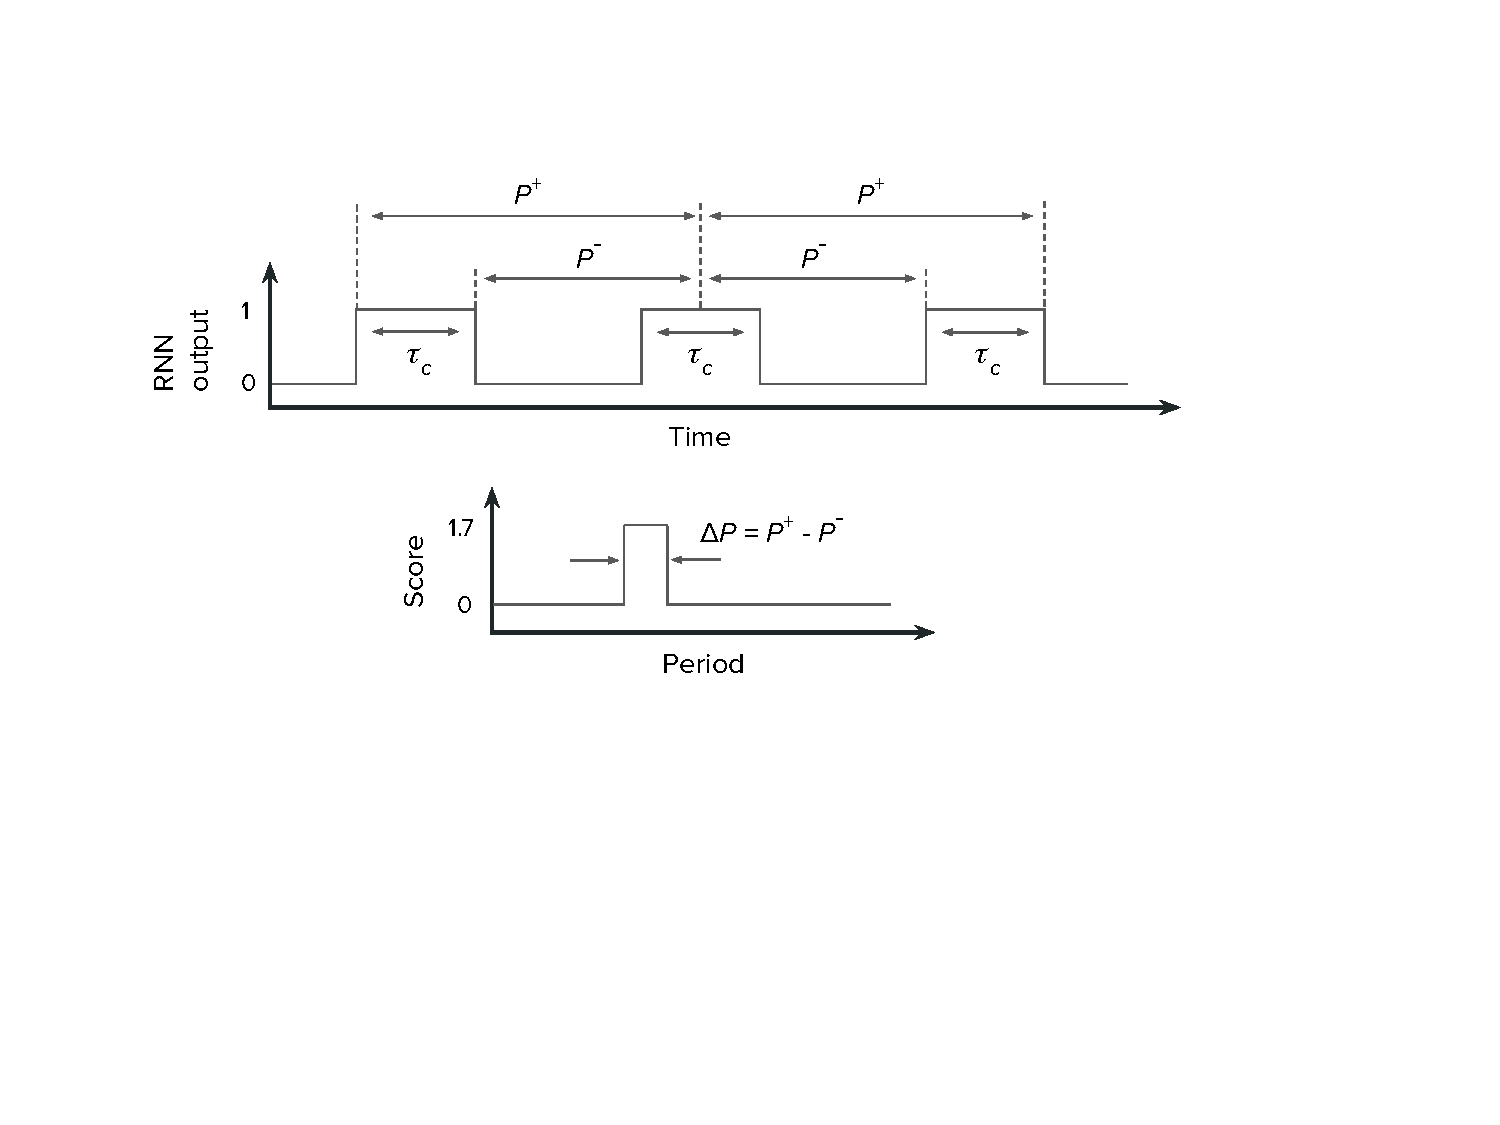
\includegraphics[width=0.6\linewidth]{Methodology/Figures/fold_drawing.pdf}
    \caption{\todo{caption}}
    \label{fig:fold_drawing}
\end{figure}

\chapter{Experiments and results}
\label{chap:experiments}

In order to better understand and evaluate the individual components of our algorithm, the first sections of this chapter are devoted to take a closer look at each one of them. We compare the RNN with the more commonly used CNN in a binary classification task for input light curve segments, and illustrate how the RNN naturally extends to full-length light curves. In the same section, Section \ref{sec:exp_hybrid}, we also motivate the network architecture that was used throughout the rest of the experiments. Since preprocessing can be of influence on the performance of the network, in Section \ref{sec:exp_preprocessing} we compare the effect of several different preprocessing steps on training of the network. For example, several approaches to dealing with gaps are evaluated, as well as the use of a generative network which is trained to fill gaps by itself.
Section \ref{sec:exp_algorithm} illustrates the workings of both detection algorithms described in Section \ref{sec:algorithms}, where success and failure cases are identified. In addition to these algorithms, we illustrate how the network's representations of each time step can be used to potentially resolve ambiguities in the matching of individual signals when searching for periodicities. 

In the last three sections, we evaluate our method as it would be used in real-world applications. First, we show that the RNN has a large potential in the task of monotransits detection. Subsequently, we compare our RNN-based detection algorithm with the BLS algorithm in the task of detecting single planets in LCSim light curves. Lastly, in the task of detecting arbitrarily many planets in more realistic light curves from Lilith-4, we compare the detections from the TESS pipeline, BLS and our method. 

\section{Detection or identification: RNN as hybrid}
\label{sec:exp_hybrid}

Without changes to the model or the training process, the RNN can be used for both the identification task and the detection task. This is illustrated in the following subsections. First, the RNN is compared against an MLP and CNN in the task of classifying light curve segments as signal or non-signal. Then, we show how the RNN trained for this task can also be used for locating signals in time for arbitrarily sized input light curves. Different network architectures are tested, which serves as a motivation for our choices of the network architecture used in subsequent experiments.

\subsection{Fixed input size, single output}
\label{sec:identification}

As described in Section \ref{eq:objective}, the RNN is trained to classify each data point of a given light curve as signal or non-signal. Recall that we refer to these outputs as the probability time series (PTS). However, in the task of classifying an entire input light curve segment as signal or non-signal, we only need a single output. Two options to obtain a single RNN output for a given input light curve segment are: (i) use the maximum of the PTS for the binary classification of the whole segment; or (ii) train an RNN specifically for this task, while only using the output at the last time step for the binary classification of the segment. We refer to (ii) as the \textit{naive} approach, since this approach does not utilize the full learning potential of the RNN as it only provides a sparse learning signal. 

Two data sets were generated using LCSim, both consisting of 15000 light curve segments for training, 5000 for validation and 5000 for testing. For each split, 50\% of the segments contained at least one transit signal and the other 50\% contained no signals. One data set contained light curve segments consisting of $N=500$ data points, and for the other data set $N = 1500$. In other words, the time spans of segments in each data set were 16.7 and 50 hours respectively. Several models were trained using the training sets, their architectures were determined by inspecting their performances on the validation sets, and only here analyse the performances on the test sets. For each model, an informal search over hyperparameters was performed to determine the final architecture, the process of which is further described in the following.

The MLP is a simple network consisting of several fully-connected (FC) layers. We experimented with different numbers of layers and nodes per layer, and decided on a network consisting of three hidden layers with 128, 64 and 64 nodes respectively. Several variations to these values were tested, but resulted in similar performance. However, the weight decay parameter seemed to be of importance to the performance of the network, as for low values of this parameter the MLP was found to quickly overfit the training data. We therefore used a weight decay of \num{5e-3}. The ReLU activation function is applied between layers and the sigmoid is applied to the final output. Each of the described networks in the following use the same activation functions.

The CNN requires the specification of more hyperparameters. In an attempt of keeping the architecture simple, we found several hyperparameter settings to result in similar performance. In the following we use a CNN with three convolutional layers, consisting of 4, 12 and 1 channels respectively, using kernel sizes of 7, 7 and 3 and a stride of 1 at each layer. After each layer, we apply batch normalization and a max-pooling operation over 3 nodes. The final layer of the network is an FC-layer of 48 nodes. 

For the RNN, GRU was found to produce better and more stable results than LSTM. In Figure \ref{fig:hybrid-gru_architectures} we compare several architectures of the bidirectional GRU with a single layer (bi-GRU-1). The hyperparameters that were varied over were the number of hidden nodes in the recurrent cell, the number of FC-layers that follow the recurrent layer, and the number of nodes per FC-layer. For each set of parameters, the network's performance on this task was similar. For each RNN tested in following experiments, we use recurrent cells with 64 hidden nodes, and two FC-layers of 64 nodes.

\begin{figure}
    \centering
    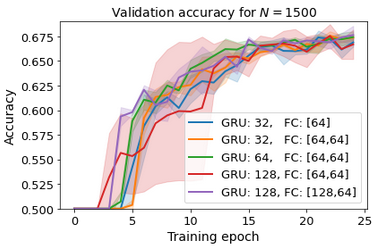
\includegraphics[width=0.4\linewidth]{Experiments/Figures/Hybrid/hybrid_architectures_identification.png}
    \caption{\red{[TODO: caption]}}
    \label{fig:hybrid-gru_architectures}
\end{figure}

\red{[TODO: provide table with test results]}
The classification accuracies of each model evaluated on the validation set during the process of training are plotted in Figure \ref{fig:hybrid-model_comparison}, from which several things can be noted. First of all, each model seems to perform worse in the case of longer ($N=1500$) light curve segments. This is probably due to the fact that the longer the segments, the more distracting background patterns may be present that mimic transit signals. The best performing models are GRU-based networks, which were not even trained for this specific task. The RNN that was trained specifically for this task, with a training procedure referred to as \textit{naive}, performed considerably worse. This is in line with our expectation that only providing a single learning signal to the RNN for a given input segment is bad practice. Lastly, we find that using more than one recurrent layer does not necessarily lead to better results. Therefore, in following experiments, we adopt a bidirectional GRU with a single recurrent layer (bi-GRU-1) that was trained on the data set with $N=1500$, and refer to this network simply as the "RNN".

\begin{figure}
    \centering
    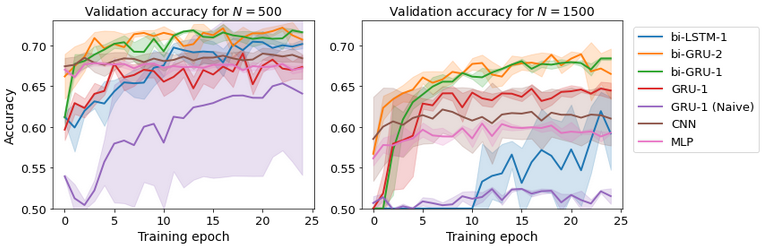
\includegraphics[width=0.8\linewidth]{Experiments/Figures/Hybrid/identification_models.png}
    \caption{\red{[TODO: caption]}}
    \label{fig:hybrid-model_comparison}
\end{figure}

\subsection{Locating signals in time for inputs of arbitrary size}

As opposed to the CNN and MLP, the RNN can handle arbitrary input sizes. This is illustrated in Figure \ref{fig:hybrid-pts}, where the RNN from Section \ref{sec:identification} is applied to a full-length light curve. In this case we show the RNN's output at each individual time step. Each peak in the resulting PTS indicates the presence of a potential transit signal at the corresponding time in the light curve. 

\begin{figure}
    \centering
    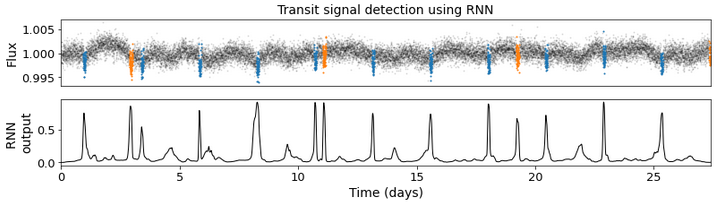
\includegraphics[width=0.8\linewidth]{Experiments/Figures/Hybrid/PTS_example.png}
    \caption{\red{[TODO: caption]}}
    \label{fig:hybrid-pts}
\end{figure}

However, data in the task of detection is less balanced than in the task of identification. This is because at the level of individual data points, we only have a few points that are labeled as signal, and many points that are labeled as non-signal. The accuracy of classification is therefore a misleading metric, as the network could already achieve high accuracies by classifying each data point as non-signal. Therefore we turn to different metrics for finetuning the network for detection. The true positive rate (TPR), or recall, is the fraction of the correctly classified positives (i.e. points labeled as signal). The true negative rate (TNR) is similar, but for correctly classified negatives instead of positives. Lastly, precision is the fraction of the samples classified as positive that were correct. 

If the classes were perfectly balanced, we expect a TPR similar to the TNR. In our LCSim data set with $N=1500$, we have 12.6 times more non-signal data points than points that are labeled as signal. Using an extra weight in the loss for transit points of $p_t=12.6$ will therefore balance our data set. Figure \ref{fig:hybrid-weighting} shows that this indeed the case. However, although tuning the TPR and TNR can be useful for our purposes, a lower TNR also means we falsely classify more samples as positive, thus decreasing the precision. To increase the recall, but avoid a large decrease in TNR we therefore adopt a smaller weight of $p_t=4$. The other weighting parameter that is varied, $w_i$, is used to tune how much each individual transit signal is weighted compared to others. For example, we can set $w_i = \delta_i / \sigma$, which will weigh each positive data point by its corresponding transit depth $\delta_i$ relative to the time-independent noise $\sigma$. In that case, a transit with twice the depth will get double the weight. This type of weighting might, however, cause the network to place too little focus on correctly detecting shallow transits. To reduce this effect, but still apply transit-specific weighting, we can adopt $w_i = \sqrt{\delta_i / \sigma}$. 


\begin{figure}
    \centering
    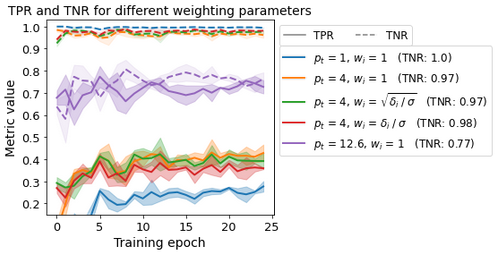
\includegraphics[width=0.5\linewidth]{Experiments/Figures/Hybrid/weighting_valid_lcsim.png}
    \caption{\red{[TODO: caption]}}
    \label{fig:hybrid-weighting}
\end{figure}

\begin{figure}
    \centering
    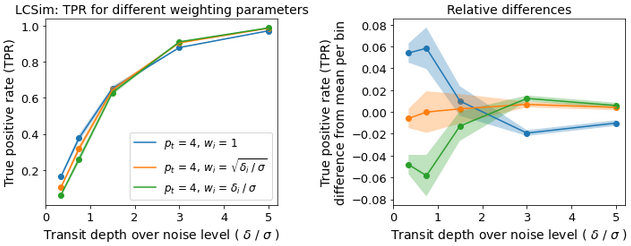
\includegraphics[width=0.65\linewidth]{Experiments/Figures/Hybrid/weighting_lcsim.png}
    \caption{\red{[TODO: caption]}}
    \label{fig:hybrid-lcsim_weighting}
\end{figure}

\begin{figure}
    \centering
    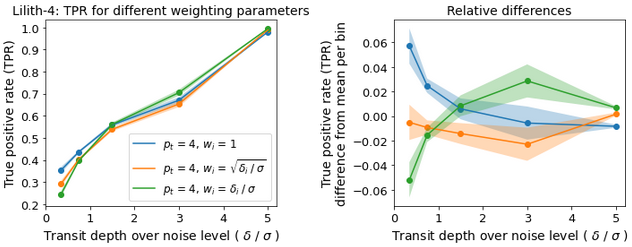
\includegraphics[width=0.65\linewidth]{Experiments/Figures/Hybrid/weighting_lilith.png}
    \caption{\red{[TODO: caption]}}
    \label{fig:hybrid-lilith_weighting}
\end{figure}

The effect of different weighting schemes on TPR and TNR are visualized in Figure \ref{fig:hybrid-weighting}. Figures \ref{fig:hybrid-lcsim_weighting} and \ref{fig:hybrid-lilith_weighting} show the TPR against different relative transit depths, which was evaluated of test splits both data sets.
\todo{describe how Lilith-4 light curve segments were obtained.} In the following experiments, we adopt $p_t=4$ and $w_i = \sqrt{\delta_i / \sigma}$, unless stated otherwise.



\section{Preprocessing and performance}

We assume the light curves segments are obtained from a median normalized light curve, e.g. by splitting the original light curve into equally sized parts. Assuming for now that no gaps are present in these segments, several additional preprocessing steps can be considered. One approach is to center the segments around zero by subtracting 1 from the flux values, and doing nothing else. Additionally, one could scale the light curves by their estimated noise level $\sigma$, so the network performance becomes less dependent on this noise and instead more on the transit depth relative to this noise. We refer to the latter step as sigma scaling, and adopt this in following experiments.  See figures \ref{fig:preprocessing-scaling_lcsim} and \ref{fig:preprocessing-scaling_lilith} for the effect of these basic preprocessing steps on the performance of the network during training. \todo{mention that each all data is standardized as last preprocessing step}

\begin{figure}
    \centering
    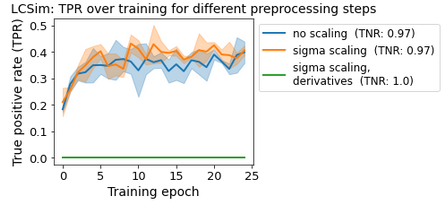
\includegraphics[width=0.5\linewidth]{Experiments/Figures/Preprocessing/preprocessing_lcsim_valid.png}
    \caption{\todo{caption}}
    \label{fig:preprocessing-scaling_lcsim}
\end{figure}

\begin{figure}
    \centering
    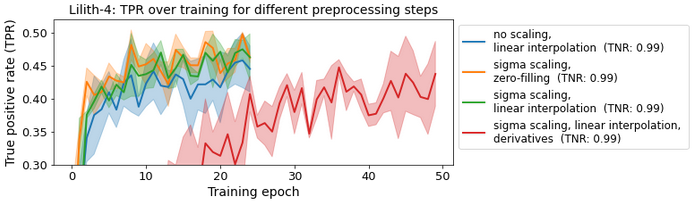
\includegraphics[width=0.75\linewidth]{Experiments/Figures/Preprocessing/preprocessing_lilith_valid_2.png}
    \caption{\todo{caption}}
    \label{fig:preprocessing-scaling_lilith}
\end{figure}

In both cases however, the range of flux values might still greatly vary between two separate light curve segments. This is understood by realizing that the original light curve may contain large-scale fluctuations due to stellar rotation modulation. The network might interpret these range differences as indicators of the presence of a transit signal, in particular if there is little data available for a certain range of flux values. This is not what we want, because a transit event can occur at any given time, independent from the activity on the stellar surface. This potential problem is visualized in Figure \ref{fig:preprocessing-ranges}.

\begin{figure}
    \centering
    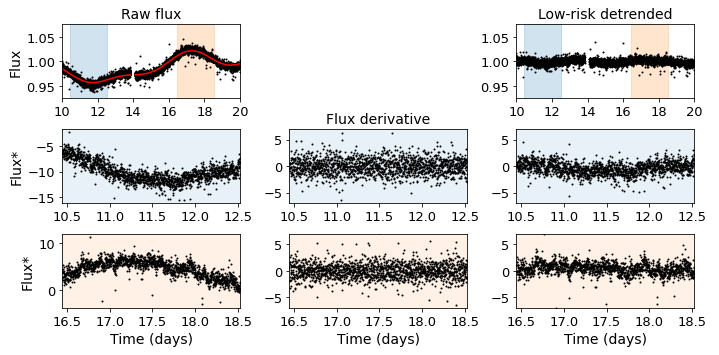
\includegraphics[width=0.8\linewidth]{Experiments/Figures/Preprocessing/prepocessing_ranges_example.png}
    \caption{\todo{caption}}
    \label{fig:preprocessing-ranges}
\end{figure}

We consider two approaches to resolve this issue: (i) feed the differences between flux values to the network, instead of their absolute values, and (ii) remove large-scale patterns from the original light curve, a process we will refer to as low-risk detrending (LRD). Both approaches have the desired effect of making the input ranges more consistent, with some exceptions. The benefits of (i) are that this approach can be applied to the segments directly and we lose almost no information by doing so. However, although all the information is still there, the structure of the data is completely changed which might be difficult for the network to learn. For (ii), we need to alter the original light curve prior to splitting it into segments. By doing so we lose information, but the result is more intuitive than (i).

In Figure \ref{fig:preprocessing-general_lilith} we compare the effect of several different preprocessing steps on the performance of the network trained on Lilith-4 data. In addition to the ``basic preprocessing'' and the ``low-risk detrending'' as described above, several other approaches are included in the comparison. For example, ``high-risk detrending'' means the input light curves are detrended such that both large and short-scale patterns are removed. This is referred to as high-risk as it comes with more risk of partly removing transit signals. The detrending filter we use for this is a time-windowed median filter with a window of 12 hours. Since real-world data may include outliers, we also evaluate the effect of removing these from the data. Outliers are identified after the light curve is detrended with a time-windowed median filter with a window of 30 minutes. Positive outliers at more than 6 standard deviations from the median and negative outliers at more than 12 standard deviations from the median are removed from the original light curve. The detrending step and the low negative-outlier threshold are to avoid transit signals from being flagged s outlier. Lastly, since Lilith-4 provides centroid data, which we also have access to for real-world data, we test the effect of using these as additional input to the network. This means that the network input at each time step consists of three values: the flux, and two values that specify the pointing of the telescope at that time step. Before use, we center the centroid data around zero, and scale them similarly to their corresponding light curve. Subsequently all the centroids in the data set are standardized independently from the flux values. This way of preprocessing is to ensure that the relative scale between light curves and their corresponding centroid data is not altered, as this might contain relevant info for the network. The series of centroid data are split into segments together with their corresponding light curve.

The results show that outlier removal had a negative influence on the performance of the network. This was unexpected, because outliers are not expected to carry relevant information. After all, an outlier should be present regardless of whether a transit event is occurring, unless the transit itself is flagged as outlier. This is unlikely to be the case, as we observe worse performance for both deep and shallow transits. We expect therefore that the reason for this result lies in the fact that outlier removal creates missing data. Missing values were imputed for this experiment, which might have caused the network to perform worse in this case. All other preprocessing steps seem to produce similar results. This is noteworthy, as the network therefore does not have to rely high-risk detrended data, as opposed to other common detection methods. 

Lastly, since Figure \ref{fig:preprocessing-general_lilith} does not clearly indicate whether or not using centroid data is beneficial, we take into consideration the results obtained on the validation set created from Lilith-4. These results, shown in Figure \ref{fig:preprocessing-general_lilith_valid}, do indicate a potential benefit of including the centroids as input to the network. This motivated us to adopt LRD as standard preprocessing procedure in combination with using centroid inputs when applying our network to Lilith-4 data in following experiments. 

\begin{figure}
    \centering
    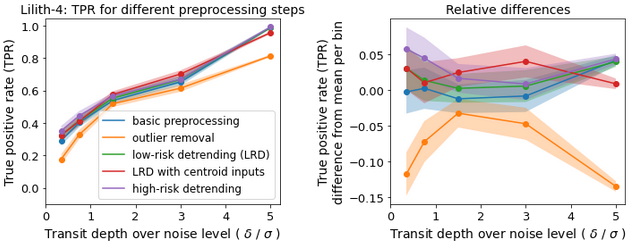
\includegraphics[width=0.65\linewidth]{Experiments/Figures/Preprocessing/test_lilith_pp.png}
    \caption{\todo{caption}}
    \label{fig:preprocessing-general_lilith}
\end{figure}

\begin{figure}
    \centering
    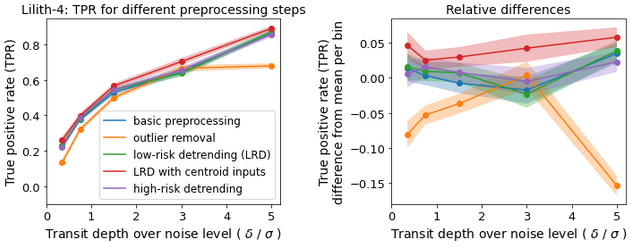
\includegraphics[width=0.65\linewidth]{Experiments/Figures/Preprocessing/validation_lilith_pp.png}
    \caption{\todo{caption}}
    \label{fig:preprocessing-general_lilith_valid}
\end{figure}

Lastly, we address the problem of missing data in greater depth. Lilith-4 data already contains data gaps, which we filled by linear interpolation up to this point, unless stated otherwise. For LCSim light curves, we manually inject NaN values in the pre-generated light curve segments to simulate data gaps. For each data split, 35\% of the samples was injected with one large data gap ranging from 2 to 10 hours, and 15\% was injected with two large data gaps. Apart from the larger gaps, each data point was replaced by a NaN value with 2\% probability. 

Three different approaches to handling gaps are evaluated. In each of the approaches, we impute the data in a different way. First, we consider replacing all missing values with zeros in the centered light curve segment. This is equivalent to replacing missing values with ones in the non-centered light curve. In the second approach, we fill the gaps by linear interpolation. When doing this, we linearly interpolate the trend of the light curve, rather than the raw flux values at the edges of a gap. The reason why we do not use the raw flux instead, is that an extreme value or outlier next to a gap could result in an apparent jump in the flux over consecutive points if it is used for interpolation. Lastly, we use the generative network as described in Section \ref{sec:extension_gen} to fill in gaps as it steps through the light curve. An example of each of the approaches is visualized in Figure \ref{fig:preprocessing-gap_examples}. 

\begin{figure}
    \centering
    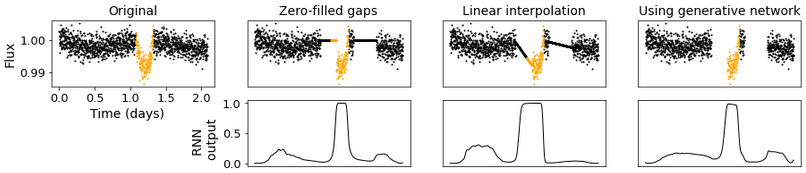
\includegraphics[width=0.8\linewidth]{Experiments/Figures/Preprocessing/gaps_example.png}
    \caption{\todo{caption}}
    \label{fig:preprocessing-gap_examples}
\end{figure}

The generative network seems to work as intended by inspecting Figure \ref{fig:preprocessing-gap_examples}. We can take a closer look at what this network is doing in Figure \ref{fig:preprocessing-generative_example}. The network is bidirectional, so we get two streams of predictions. We can see that these can complement each other. If we only consider the predictions from left-to-right in the first gap and from right-to-left in the second, then the missing values are well reconstructed. However, since each unidirectional component of the network has no information of what comes after a gap, we see the predictions drift off to unrealistic values.

\begin{figure}
    \centering
    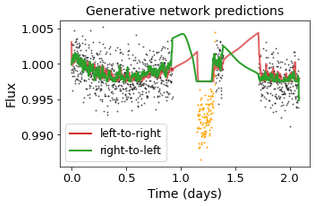
\includegraphics[width=0.34\linewidth]{Experiments/Figures/Preprocessing/generative_example.png}
    \caption{\todo{caption}}
    \label{fig:preprocessing-generative_example}
\end{figure}

After evaluation on the gap-injected test set, of which the results are presented in Figure \ref{fig:preprocessing-gaps_lcsim}, we find that each approach to handling gaps leads to similar network performance in terms of TPR, at the same value for TNR. However, on average linear interpolation seems to work slightly better than the other approaches, which we therefore use in following experiments.

\begin{figure}
    \centering
    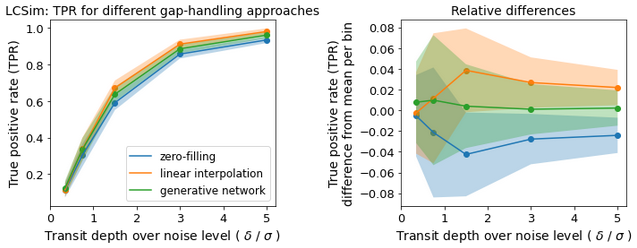
\includegraphics[width=0.65\linewidth]{Experiments/Figures/Preprocessing/pp_gaps_lcsim.png}
    \caption{\todo{caption}}
    \label{fig:preprocessing-gaps_lcsim}
\end{figure}

\section{Algorithm comparison: searching for periodic signals}
\red{[TODO]}

\section{Monotransit retrieval}
\red{[TODO]}

\section{Single planet retrieval}
\label{sec:singles}

For the evaluation of the ability of the RNN-based algorithms to retrieve single planets with multiple transit signals, we apply the RNN from previous sections to light curves in the LCSim-Single data set. Subsequently, we use PTS-Fold and PTS-Peak to determine the period and epoch of a maximum of three candidate signals per light curve. Both algorithm give each candidate a corresponding score, as described in Section \ref{sec:algorithm}, which is used to set a detection threshold. A detection is counted as correct if the estimated period is correct with a 1\% error margin, and the estimated epoch is within the duration of the first transit in the light curve.

As baseline we use the standard BLS algorithm, as implemented in the \texttt{astropy} package\footnote{\url{https://docs.astropy.org/en/stable/timeseries/bls.html}}. We set a detection threshold on the SDE of each candidate in the BLS periodogram, and recursively apply the method to search for a maximum of three potential signals per light curve, each time masking the previous signal that was found. The algorithm is applied to detrended light curves using sliding median filters of varying lengths (6, 12, and 24 hours).

Figure \ref{fig:single_pr} shows that a 12-hour window works best for detrending in combination with BLS for this task, which is in line with the results from \cite{hippke2019wotan}. Moreover, the results show that the BLS algorithm outperformed the RNN-based detection algorithms in this experiment. Among the RNN-based algorithms tested, PTS-Fold performed best, which was as expected because it does not rely on distinct peaks in the PTS as opposed to PTS-Peak. The performance of the best performing algorithms can is further inspected in Figure \ref{fig:single_transit}. This figure shows, in line with our monotransit experiment, that towards larger periods, i.e. fewer transit signals, the performance of BLS drops faster than that of the RNN-based algorithm. This suggests that if there is periodicity in the signal, BLS remains dominant over the RNN. However, if the periodicity is lacking, the RNN is the preferred method. Table \ref{tab:single_AnotB} presents the number of planets retrieved by the methods, including the number of planets that were not found by one method and not by the other.

The RNN-based algorithm required a longer computation time in this case than in the monotransit case. To obtain the PTS of each of the 5000 light curves still required only a few minutes on a GPU, but the determination of the periodicity of potential signals added more to the necessary computation time. PTS-Peak required only required 5 minutes on a CPU. PTS-Fold on the other hand, took about 1.5 hours. Still, PTS-Fold was faster than BLS with over 3 hours of computation time. The computation times are in line with the relative performances of each method in this task. 


\begin{figure}
    \centering
    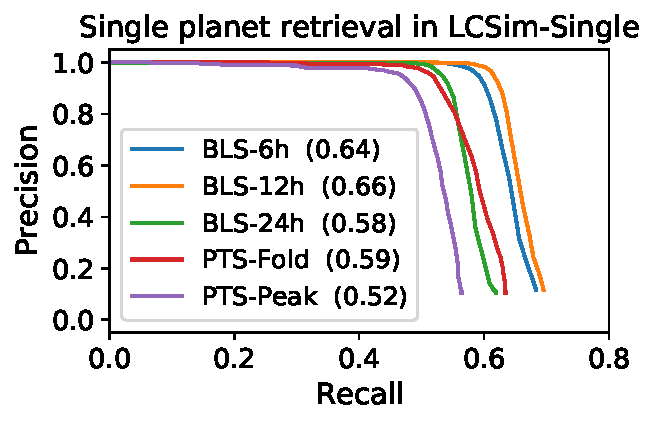
\includegraphics[width=0.35\linewidth]{Experiments/Figures/Singles/single_pr.pdf}
    \caption{Precision-recall curves for different methods in the task of detecting repeating transit signals of a single planet. The average precision is given between brackets.}
    \label{fig:single_pr}
\end{figure}


\begin{figure}
    \centering
    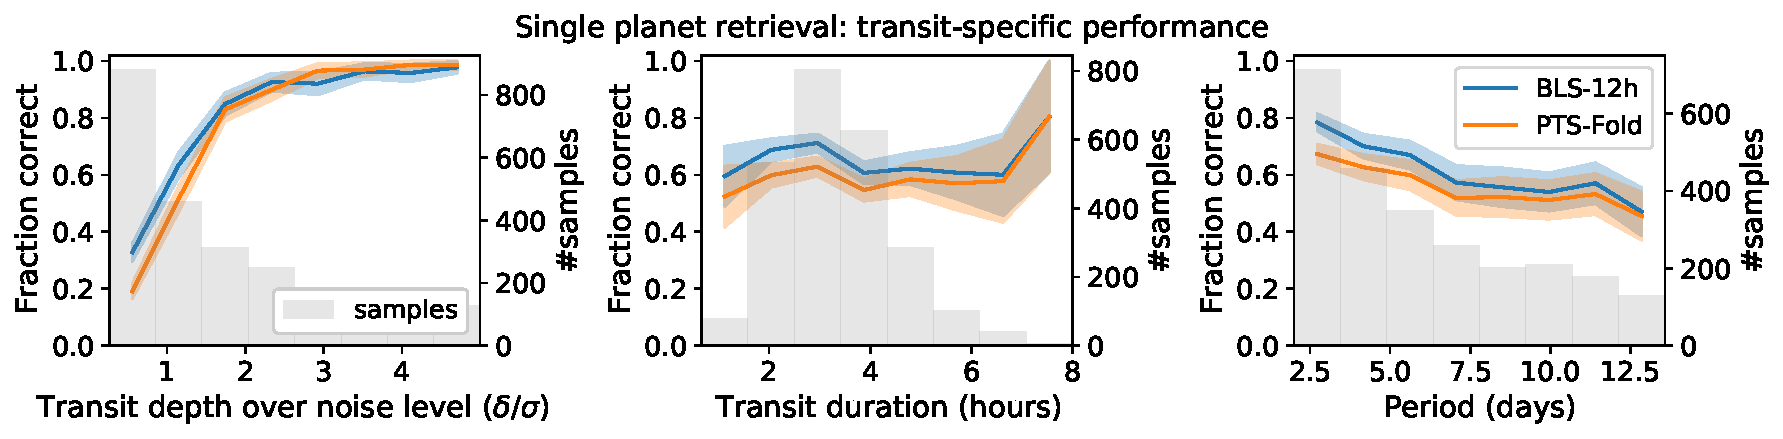
\includegraphics[width=\linewidth]{Experiments/Figures/Singles/single_transit_specific.pdf}
    \caption{The ability of the presented methods to retrieve planets within the given parameter ranges. A detection threshold was set closest to a corresponding detection precision of 0.5. PTS-Peak is not shown because it behaves similarly but worse than PTS-Fold and would therefore only clutter the image. Filled regions show the Wilson score interval \citep{wilson1927probable}, which approximates the 95\% confidence interval of the performance per bin.}
    \label{fig:single_transit}
\end{figure}



\begin{table}[h]
\label{tab:single_AnotB}
\centering
\begin{tabular}{@{}lrlrlrl@{}}
\toprule
             & \multicolumn{2}{c}{PTS-Fold} & \multicolumn{2}{c}{PTS-Peak} & \multicolumn{2}{c}{BLS-12h} \\ \midrule
             & 1480      & (1.00, 0.59)     & 1333      & (1.00, 0.53)     & 1655     & (1.00, 0.66)     \\
not PTS-Fold & -         &                  & 7         & (0.01, 0.00)     & 224      & (0.14, 0.09)     \\
not PTS-Peak & 154       & (0.10, 0.06)     & -         &                  & 342      & (0.21, 0.14)     \\
not BLS-12h  & 49        & (0.03, 0.02)     & 20        & (0.02, 0.01)     & -        &                  \\ \bottomrule
\end{tabular}
\caption{The absolute and relative number of correct detections in the task of retrieving planets with multiple transit signals, where the detection thresholds are set closest to a corresponding detection precision of 0.5.  The data contained a total of 2500 planets.}
\end{table}
\section{Multiplanet retrieval}
\label{sec:multis}

Similar to the single planet case, we compare the RNN-based detection algorithms with BLS in the task of retrieving planets with multiple transit signals. In this case we use Lilith data, which in some cases contain transit signals from different planets within the same light curve. Again we restrict both methods to only output three candidate detections per light curve, to save on computation time.

In this experiment we also include the TESS pipeline detections for the given data set. However, since a threshold has already been set on the pipeline detections, we only have limited data, and the PR-curve for the pipeline therefore cannot be drawn fully. For the pipeline's PR-curve shown in Figure \ref{fig:multi_pr}, we set a threshold on the SNR of the detections that are provided in the DV files. It can be seen from this figure, that the pipeline's PR-curve steadily decreases, suggesting that a high AP could be obtained if we had access to all the detections below the pre-set threshold. In contrast, the RNN-based algorithms drop down steeply. Nevertheless, the RNN-based methods seem to be able to maintain high precision for the detection of about 10\% of all the planets. BLS on the other hand, starts off with relatively low precision, but is able to retrieve far more of the total number of planets. In terms of average precision, it therefore outperformed the other methods. Figure \ref{fig:multi_transit} shows the detection results over the distribution of transit samples for different parameters. We can see that each method behaves similarly, but at different levels of performance. Table \ref{tab:multi_AnotB} presents the number of planets retrieved by each method, including the number of planets that were detected by one method and not by the other. Table \ref{tab:multi_AnotB} is provided to give a closer view on the ability of PTS-Fold and BLS-12h to retrieve multiple planets in a single light curve. From this table we can see that PTS-Fold is able to detect multiple planets in the same light curve, but there is room for improvement as compared to BLS-12h.

\begin{figure}
    \centering
    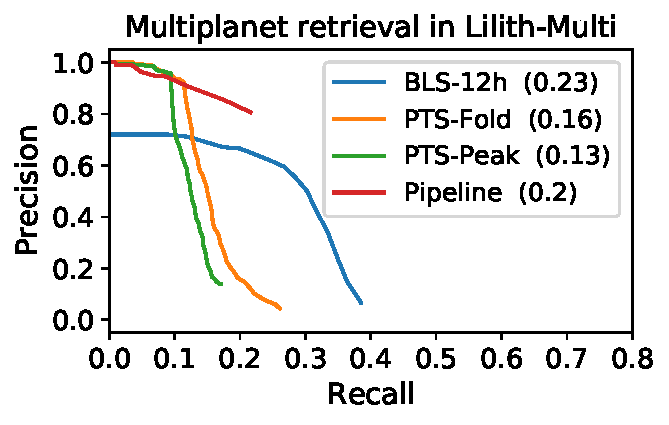
\includegraphics[width=0.35\linewidth]{Experiments/Figures/Multis/multi_pr.pdf}
    \caption{Precision-recall curves of different methods in the task of detecting repeating transit signals in light curves of Lilith-Multi. The PR-curve for the TESS pipeline could not be drawn fully due to limited available data.}
    \label{fig:multi_pr}
\end{figure}

\begin{figure}
    \centering
    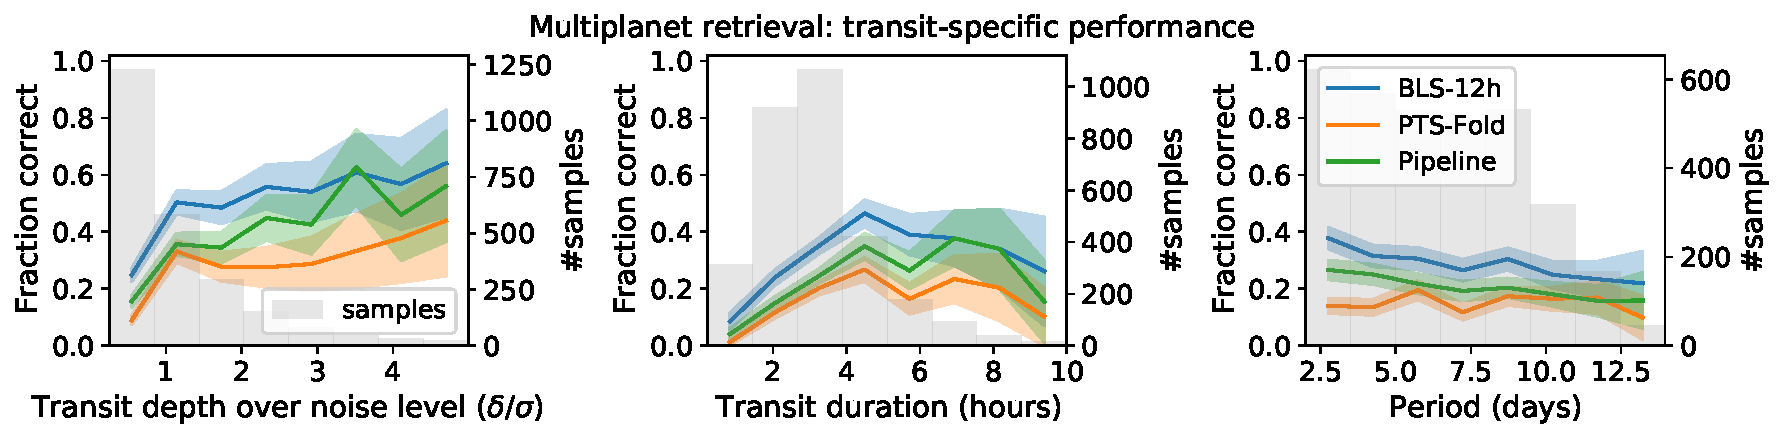
\includegraphics[width=\linewidth]{Experiments/Figures/Multis/multi_transit_specific.pdf}
    \caption{A closer look into the ability of each method to retrieve planets in the given parameter ranges. A detection threshold is set closest to a corresponding detection precision of 0.5. Filled regions show the Wilson score interval \citep{wilson1927probable}, which approximates the 95\% confidence interval of the performance per bin.}
    \label{fig:multi_transit}
\end{figure}

\begin{table}[]
\label{tab:multi_AnotB}
\centering
\begin{tabular}{@{}lrlrlrl@{}}
\toprule
             & \multicolumn{2}{c}{PTS-Fold} & \multicolumn{2}{c}{BLS-12h} & \multicolumn{2}{c}{Pipeline} \\ \midrule
             & 493      & (1.00, 0.15)      & 993      & (1.00, 0.30)     & 710      & (1.00, 0.22)      \\
not PTS-Fold & -        &                   & 522      & (0.53, 0.16)     & 304      & (0.43, 0.09)      \\
not BLS-12h  & 22       & (0.04, 0.01)      & -        &                  & 46       & (0.06, 0.01)      \\
not Pipeline & 87       & (0.18, 0.03)      & 329      & (0.33, 0.10)     & -        &                   \\ \bottomrule
\end{tabular}
\caption{The absolute and relative number of correct detections in the task of retrieving planets with multiple transit signals in Lilith data, where the detection thresholds are set closest to a corresponding detection precision of 0.5. For the pipeline, the level of precision is in fact higher and the numbers presented here are relatively small, because we had no access to its lower confidence detections. The data contained a total of 3285 planets.}
\end{table}

\begin{table}[]
\label{tab:multi_numpl}
\centering
\begin{tabular}{@{}cccccc@{}}
\toprule
\multirow{2}{*}{\begin{tabular}[c]{@{}c@{}}\# planets\\ (\# light curves)\end{tabular}} & \multirow{2}{*}{Method} & \multicolumn{4}{c}{Detected} \\
                                                                    &          & 1   & 2  & 3 & 4 \\ \midrule
\multirow{2}{*}{\begin{tabular}[c]{@{}c@{}}1\\ (2130)\end{tabular}} & PTS-Fold & 371 &    &   &   \\
                                                                    & BLS-12h  & 666 &    &   &   \\ \cdashlinelr{1-6}
                                                    
\multirow{2}{*}{\begin{tabular}[c]{@{}c@{}}2\\ (474)\end{tabular}}  & PTS-Fold & 80  & 9  &   &   \\
                                                                    & BLS-12h  & 120 & 65 &   &   \\ \cdashlinelr{1-6}
                                                    
\multirow{2}{*}{\begin{tabular}[c]{@{}c@{}}3\\ (57)\end{tabular}}   & PTS-Fold & 13  & 5  & 0 &   \\
                                                                    & BLS-12h  & 8   & 20 & 6 &   \\ \cdashlinelr{1-6}
\multirow{2}{*}{\begin{tabular}[c]{@{}c@{}}4\\ (9)\end{tabular}}    & PTS-Fold & 1   & 0  & 0 & 0 \\
                                                                    & BLS-12h  & 4   & 2  & 1 & 0 \\ \bottomrule
\end{tabular}
\caption{The number of correctly detected planets per light curve with a given number of planets in Lilith data. For example, of the 57 light curves that contained 2 planets, PTS-Fold was able to retrieve 2 planets from 5 light curves, and only 1 planet from 13 light curves.  The detection threshold was set closest to a corresponding detection precision of 0.5. We can see that BLS-12h is better able to detect multiple planets in the same light curve than PTS-Fold.}
\end{table}


\chapter{Discussion}
\label{chap:discussion}

The main questions in thesis were whether and how RNNs could be used for the detection of transit signals, and whether they provide a competitive and efficient alternative to existing approaches. In addition, we attempted to investigate how the outputs of the RNN could be made more interpretable for this task, such that it would benefit the transit detection algorithm. In the following, we discuss these questions with regard to the results presented in Chapter \ref{chap:experiments}. The subsequent sections describe the limitations of this work and directions for future work.

\section{Answers to research questions}

One of the goals of this research was to assess whether and how RNNs could be applied for the task of transit signal detection. Although this work is only based on simulated data, the results achieved on both LCSim and Lilith data show that RNNs have promising capability of performing well in this task. 

The question of how RNNs should be applied for this task was investigated in several experiments. Different preprocessing steps were considered, for example about how data gaps are handled or the way the input data is scaled. Although RNNs come with the possibility of predicting missing values in a light curve, we found that a simple gap-filling approach such as linear interpolation leads to similar results, while requiring less computation time. Regarding the scaling of light curves prior to applying the RNN, we expected that scaling light curves by their estimated white noise level would be beneficial to the network. This was because in that case, the level of white noise cannot be seen as feature and only the depth of a transit signal relative to this noise would stand out. However, the results showed that this sort of scaling, which we referred to as sigma scaling, did not have a large effect on the result, and measuring its impact on the detection performance was therefore difficult. What we were able to measure, was the effect of applying low-risk detrending to remove only large scale stellar variability, with the goal of making the input ranges to the network more consistent. This way of detrending proved to be beneficial for the RNN applied Lilith light curves, while the more standard way of (high-risk) detrending did not improve the results. Centroid data also seemed to help the network to distinguish background patterns from data points belonging to transit signals.

In addition to preprocessing, the network architecture and training played a large role in our transit detection algorithm. It was shown how using different weighting parameters in the network's loss function, can help finetune the network for the unbalanced task which we are dealing with. For example, it was found that a simple positive weight, which gives extra weight to the predictions over data points belonging to transit signals, can help in shifting the tradeoff between precision and recall that can be made at given classification thresholds. We expect that this weight helps to increase the noise floor in the PTS for a given light curve, which we found to be higher for LCSim data than for Lilith data. Since the noise in the PTS may still contain relevant information about the precence of potential signals, a larger positive weight for Lilith data may have resulted in higher recall for the RNN-based detection algorithms. A transit-specific weight was also adopted, with the desired effect of balancing the network's focus of learning to detect transit signals of varying depths. 

Regarding the network architecture, we opted for a relatively simple design. In the first place, this was to illustrate that this task does not require a highly complex network architecture. In addition, a simple architecture would allow for easier reproduction of the work. During the process of comparing architectures, in fact we found that simpler architectures improved over more complex ones. For example, GRU produced better and more stable results than LSTM, while having less parameters. Furthermore, a network with multiple recurrent layers performed slightly worse than the simpler network with only one layer. Including bidirectionality in the RNN on the other hand, lead to a great improvement in the results. The confidence RNN only slightly more complex than the basis network, but also resulted on worse overall performance.

Apart from how the network should be applied, we sought to answer the question of whether an RNN-based transit detection algorithm provides an efficient and competitive alternative to existing approaches. In terms of efficiency, neural networks in general are appealing compared to the common brute-force approach that is taken to search for transits. The computation times observed in the experiments for Mono-BLS and BLS compared to our RNN-based approach were in line with this expectation. Among different types of NNs, RNN is known to be less efficient than the CNN, due to its recurrent structure. However, since CNNs are required to be applied multiple times to the same light curve in the task of transit detection, this difference becomes smaller. A comparison of efficiency between the two methods has not been made in this work,  because many different design choices of this way of using the CNN could lead to different results. For typical TESS light curves of 27.4 days, our RNN was able to compute the PTS in under one second for over 50 light curves at once. This is reassuring, because the data sets that are currently produced by TESS and in the future by PLATO require efficient algorithms. The most time was taken by the method which determines the periodicity of candidate signals using the PTS. In this task, PTS-Fold lead to more correct detections than PTS-Peak, but PTS-Peak outperformed PTS-Fold in terms of effeciency by at least one order of magnitude. This is because PTS-Fold tends more towards a blind search, while PTS-Peak is guided by the detection of individual events in the PTS. If the search is directed towards monotransits, however, we do not require PTS-Fold or PTS-Peak, and the PTS can directly be used to set detection thresholds. For this reason, the search for monotransits in large data sets can be conducted in minutes.

Not only in terms of efficiency, but also in terms of detection performance, the RNN showed most potential in the case of montransits. We found it to be more robust against transit-resembling noise patterns than a box fitting aproach. This is likely because it was specifically trained on individual transit signals, and not on aggregated or folded light curves. It therefore does not rely on periodicities of signals, the way BLS does. BLS uses periodicities to its advantage,  by aggregating multiple transits in the same light curve, effectively increasing the SNR of the signal. We expect this to be the reason that BLS was still dominant in the case of repeating signals. Nevertheless, we found multiple examples of where BLS failed to detect a planet, while the RNN was able to detect it. Some of these cases showed to be highly noisy light curves with noise patterns at time scales similar to the transit signal. In these cases, detrending may be the limiting factor for BLS to detect the planets. Since the RNN does not require detrending, it may still distinguish the signals from the distracting background.

Lastly, we raised the question of whether the outputs of the RNN could be made more interpretable. Althoug true uncertainties are difficult to obtain, we attempted to let the RNN output an indication of its confidence over given outputs. Visually, the results were as we would expect: in noisy regions of a light curve the confidence often was slightly reduced, even though the standard outputs remained the same; in the case of a transit signal, the confidence would be low at ingress and egress, indicating that the network is not certain when exactly the transit starts and ends. However, in many cases the confidence outputs $c$ were approximately the same as $y$ mirrored, i.e. $y = 1-c$. We expect this to be the reason why we did not observe differences in the performance if the confidence outputs were or were not used in the task of monotransit detection.

Another attempt of increasing the interpretability of the RNN outputs, involved the use of learned representations of signals. We only provided an illustration of how these representations may be used to resolve ambiguities, but the few examples that we evaluated showed intuitive results. The standard outputs of the RNN provide only limited information. Any increase in the PTS may indicate the presence of a transit signal, but sometimes it is not clear what triggers the response of the RNN. Moreover, the connection between two peaks in the PTS can only be based on their duration. Learned representations could open the door to understanding better what caused the RNN to output a certain value, by comparing its representations to other cases.  In addition, as shown in this work, they can be used to separate the detection of signals from different planets. However, more research needs to be conducted to evaluate the effectiveness of this approach.


\section{Limitations and suggestions}
\red{[TODO]}

\bullets{• simulated data != real data - though in 4.3 we provide examples using real data\\
• Lilith-4 was generated before flight (see differences (\url{https://iopscience.iop.org/article/10.3847/2515-5172/ab35e0/meta}) with real TESS data)\\
• nevertheless, simulators provide a great tool for training our method, provided good quality\\
• uncertaintainty over P, t0 not provided by the model\\
• some design choices depend on previous choices - all choices are considered in combination with each other (e.g. fully tuning each network architecture) gives more complete and reliable comparisons, but was computationally infeasible for this project\\
• transits could overlap (as described in 3.1.1.5.) - model could be able to handle this - but also it was not trained on such events, so it might get confused\\
• longest transits - need long term memory (all in-transits points classified as signal), instead one could have the model only detect ingress and egress of transit signals (begin and end), and define detections by consistent pairs - this might also help for overlapping transit }

\section{Future directions}

A clear direction for the future of the RNN-based detection method is to be applied to real-world data. Especially in the task of monotransit detection, we expect the RNN to lead to interesting new results. In our work, a general search for transits was evaluated, i.e. transits of varying depths and varying shapes. However, the training of the network can also be tuned for the search for specific kind of transit signals. For example, the training data can be injected with transits from exoplanets with orbiting ``exomoons''.  In this approach, the network can be trained to only detect these special transits, while ignoring the ``normal'' transit signals. Similarly, one could inject the training data with transits only from disintegrating rocky exoplanets (DREs), or transits signals from other particularly interesting  objects.

To address several of the limitations described in the previous section, future research could also aim at improving the detection method. For example, it would be highly favorable if the network is able to work with periodicities of potential signals, such that network directly outputs $P$ and $t_0$ and can be trained end-to-end. A considerable portion of this project was devoted to finding a solution for this, without success.  Other directions include the
estimation of more parameters in the output of the network, e.g. the depth or duration of the signal, and estimations of their uncertainties. Further research could also evaluate the effect of EB signals on the performance of the RNN. For example, either by considering EB signals as noise, or by including them in the problem as an additional class of signal.

Lastly, we found the problem of transit detection to not always be defined clearly or consistently in literature.  Therefore we believe it would be worth constructing a benchmark data set with a clearly defined task, specifically for the task of transit signal detection. Not only would this make the comparison between different papers and methods easier, it may also motivate more AI researchers to tackle this problem from different perspectives.

\chapter{Conclusions}
\label{chap:conclusions}

\red{[TODO]}

\bibliography{library} 
\addcontentsline{toc}{chapter}{References}
% \bibliographystyle{ieeetr}
\bibliographystyle{plainnat}

\appendix
\addtocontents{toc}{\protect\setcounter{tocdepth}{-1}}
\chapter{}
\addtocontents{toc}{\protect\setcounter{tocdepth}{4}}
\addcontentsline{toc}{chapter}{Appendix}

\section{Conference and workshop contributions}


This work has been communicated to the scientific community through presentations and abstracts at several international conferences and workshops. Early on in the project, the abstract titled ``Towards Deep Learning for Transiting Exoplanet Search Using Simulated TESS Data''\footnote{\url{https://www.hou.usra.edu/meetings/lpsc2021/pdf/2080.pdf}} \citep{rusticus2021towards} was submitted to and accepted by the 52nd Lunar and Planetary Science Conference (LPSC). At this conference, both a 3-minute live lightning talk and pre-recorded presentation of 15 minutes were given. At the annual meeting of 2021 of the European Astronomical Society (EAS), the abstract titled ``A Transit Detection Algorithm Based on Recurrent Neural Networks''\footnote{\url{https://eas.kuoni-congress.info/2021/programme/abstract/1918}} was accepted. This resulted in a live 15-minute presentation in the session for ``machine learning and visualisation in data intensive era''. Lastly, at several EuroMoonMars (EMM) workshops, presentations of 5-10 minutes were given for ESA scientists, students and collaborators.

\end{document}

